\documentclass[11pt,a4paper]{report}

\usepackage{amsmath, amssymb}
\usepackage{geometry}
\usepackage{parskip}
\usepackage{titlesec}
\usepackage{setspace}
\usepackage{graphicx}
\usepackage{float}
\usepackage{fancyhdr}
\usepackage[font=small,labelfont=bf]{caption}
\usepackage[ruled,vlined,linesnumbered]{algorithm2e}
\SetAlCapFnt{\footnotesize}
\SetAlCapNameFnt{\bfseries}
\usepackage{url}
\usepackage{tabularx}
\usepackage{xcolor}
\usepackage{booktabs}
\usepackage{hyperref}
\usepackage{bookmark}
\usepackage{hanging}
\usepackage{enumitem}
\usepackage{placeins}
\usepackage{textcomp}
\sloppy

\usepackage{array}
\renewcommand{\tabularxcolumn}[1]{m{#1}}
\usepackage{array}

\newcolumntype{M}[1]{>{\raggedright\arraybackslash}m{#1}}
\newcolumntype{Y}{>{\raggedright\arraybackslash}X}

\usepackage{colortbl}
\usepackage{svg}

\geometry{a4paper, margin=1in}
\graphicspath{{./}}

\numberwithin{figure}{chapter}
\numberwithin{table}{chapter}
\numberwithin{equation}{chapter}

\titleformat{\chapter}[hang]
  {\normalfont\huge\bfseries\raggedright}{Chapter \thechapter}{1em}{}
\titlespacing*{\chapter}{0pt}{-20pt}{25pt}

\titleformat{\section}
  {\normalfont\large\bfseries\raggedright}{\thesection}{1em}{}

\titleformat{\subsection}
  {\normalfont\normalsize\bfseries}{\thesubsection}{1em}{}

\setstretch{1.5}
\setcounter{tocdepth}{2}
\setcounter{secnumdepth}{3}

\hypersetup{
    colorlinks=true,
    linkcolor=blue!55!black,
    citecolor=blue!55!black,
    urlcolor=blue!55!black,
    pdftitle={F-Score on High B/M Equities with MPT Portfolio Construction across Three Equity Markets},
    pdfauthor={Ta Tan Phat, Zhicheng Ding, Zu Yao Teoh}
}

% Working-draft helpers. These can be removed before submission.
\newcommand{\placeholder}[1]{\textcolor{red}{\textbf{[PLACEHOLDER: #1]}}}
\newcommand{\working}[1]{\textcolor{blue!70!black}{\textbf{[WORKING ASSUMPTION: #1]}}}
\newcommand{\FScore}{F-Score}
\newcommand{\BM}{B/M}
\newcommand{\RMT}{RMT}

\begin{document}

\pagestyle{fancy}
\fancyhf{}
\fancyhead[L]{\scriptsize Capstone Project Members: (A) Ta Tan Phat\quad (B) Zhicheng Ding\quad (C) Zu Yao Teoh}
\fancyfoot[C]{\thepage}
\renewcommand{\headrulewidth}{0.4pt}

% =============================================================================
% COVER PAGE
% =============================================================================
\begin{titlepage}
\thispagestyle{empty}

\begin{center}

\includesvg[width=0.32\textwidth]{wqu-logo.svg}

\vspace{0.6cm}

% \textbf{WorldQuant University}\\
MSc Financial Engineering\\
MScFE 690 Capstone Project\\
Track: Quantitative Fundamentals

\vspace{1.6cm}

\Large
\textbf{F-Score on High B/M Equities with MPT Portfolio Construction across Three Equity Markets}

\vspace{1.5cm}

\normalsize
\textbf{Group Members}

\vspace{0.3cm}

\begin{tabular}{@{}c l@{}}
(A) & Ta Tan Phat (tatan.phattt@gmail.com) \\
(B) & Zhicheng Ding (mike.ding.work@gmail.com) \\
(C) & Zu Yao Teoh (computingteoh@gmail.com) \\
\end{tabular}

\vfill

August 2026

\end{center}

\end{titlepage}

\pagenumbering{roman}

% =============================================================================
% ABSTRACT
% =============================================================================
\chapter*{Abstract}
\addcontentsline{toc}{chapter}{Abstract}

This capstone studies whether Piotroski's F-Score can be used as a practical stock-selection signal inside high book-to-market equity universes, and whether portfolio construction based on Modern Portfolio Theory can improve the result after the stocks are selected. We compare three markets, the United States, Japan and Vietnam, which gives us two developed equity markets and one less-developed market setting with quite different market structure and data limitations. The common headline experiment forms portfolios every July from 2012 through 2024, holds each portfolio for one year, and therefore evaluates the common period from July 2012 through June 2025.

For each formation year, an eligible and liquid stock universe is constructed first, the top 40\% by book-to-market is retained, and the stocks are then ranked by the nine-signal Piotroski F-Score. The main portfolio size is $K=30$. We compare an equal-weight F-Score portfolio with two covariance-based constructions, a long-only global minimum variance portfolio using Random Matrix Theory denoising, and a sector-capped version of the same portfolio. The equal-weight portfolio does not use RMT because no covariance matrix is needed for equal weighting. Statistical significance is assessed using matched Monte Carlo portfolios drawn from the same annual high-B/M universe, with 1,000 equal-weight simulations and 300 simulations for each optimized construction.

The results are mixed across the three markets, which is also one of the main findings of the study. Equal-weight F-Score selection is statistically significant on return and Sharpe ratio in Japan and Vietnam, but not in the United States. In the United States, stronger evidence comes from the optimized portfolios, especially the sector-capped GMV portfolio. RMT-based optimization therefore can add value, but it does not do so in a consistent way across all markets. Overall, the evidence suggests that F-Score contains useful information, although its portfolio-level effectiveness depends on the market, the size of the opportunity set and the way the selected stocks are combined.

% =============================================================================
% ACKNOWLEDGEMENT
% =============================================================================
\chapter*{Acknowledgement}
\addcontentsline{toc}{chapter}{Acknowledgement}

A heartfelt thanks to WorldQuant University and its terrific staff, specifically Igor Tulchinsky, for providing us with a quality education in Financial Engineering and Quantitative Analytics. We also appreciate the opportunity that the MScFE program gave us to work together on a research problem that combines financial statements, portfolio theory, statistical testing, and real market data, it has been a useful way for us to put many parts of the program together in one project.

\clearpage
\tableofcontents
\clearpage
\listoffigures
\clearpage
\listoftables
\clearpage
\pagenumbering{arabic}

% =============================================================================
% CHAPTER 1
% =============================================================================
\chapter{Introduction}
\label{chap:introduction}

\section{Research Motivation}

Piotroski's F-Score is a simple accounting-based framework that tries to separate financially stronger firms from weaker firms using nine binary signals from the income statement, balance sheet and cash-flow statement. The original study was not designed as a general ranking rule for every listed company. It was developed in a high book-to-market setting, where the market may already be pricing firms pessimistically and accounting information can help distinguish companies that are financially improving from firms whose low valuation may be justified (Piotroski, 2000).

This is the basic motivation of our capstone. We want to see whether this idea can still be useful when it is taken outside the original U.S. study and applied to markets that are different from each other, and then we also want to ask another question, which is whether the stock-selection signal and the portfolio-construction problem should be treated separately because a good set of stocks does not automatically mean a good portfolio. A portfolio can contain fundamentally strong names but still be poorly diversified, highly correlated, or concentrated in the same sector.

The project therefore combines two ideas. The first is fundamental selection using high B/M and Piotroski F-Score. The second is portfolio construction using equal weighting and minimum-variance optimization, where covariance matrices used by the optimized portfolios are cleaned using Random Matrix Theory. This gives us a way to ask whether the F-Score adds information, and separately whether a more deliberate construction method changes the risk and return of the selected basket.

\section{Countries Studied and Evolution of the Project}

The original project proposal focused on the United States, Japan and Malaysia. Vietnam was later added because it gives a substantially different market environment and because a team member had access to specialized Vietnamese data sources and local market knowledge. During the data-building stage, Malaysia became difficult to maintain at the same level of completeness and point-in-time consistency as the other markets, so the final empirical study contains the United States, Japan and Vietnam only. We mention this project change briefly because it explains the final country set, but the analysis that follows is based only on the frozen three-country design.

The three markets are useful together. The United States and Japan are large developed equity markets with established institutional infrastructure, while Vietnam gives a less-developed market setting where liquidity, data availability and trading structure are quite different. We are not assuming that the same signal must work equally well in each place, actually the cross-country difference is part of what we want to learn from the study.

\section{Research Questions}
\label{sec:research_questions}

The report is organized around three main research questions:

\begin{enumerate}[label=\textbf{RQ\arabic*:}, leftmargin=1.6cm]
    \item Does Piotroski F-Score identify portfolios with superior performance within a high book-to-market opportunity set?
    \item Is the effectiveness of the F-Score reasonably consistent across the United States, Japan and Vietnam?
    \item After the F-Score basket is selected, does RMT-denoised minimum-variance portfolio construction improve its risk-adjusted performance relative to a simple equal-weight construction?
\end{enumerate}

The first question is mainly about stock selection. The third one is different because RMT does not enter the equal-weight portfolio at all, it only enters the covariance-based GMV portfolios. We make this separation explicit throughout the report because otherwise it becomes easy to talk about ``RMT portfolios'' as if every F-Score portfolio is using RMT, which is not the case.

\section{Main Contribution of the Study}

The contribution of this capstone is not to claim a new universal factor. The goal is more practical. We build one comparable annual framework across three different markets, preserve the high-B/M setting that motivated Piotroski's original work, use point-in-time accounting rules to avoid using future information, and compare the selected portfolios with matched random baskets instead of only comparing them with an index. The Monte Carlo comparison is useful because it asks whether the F-Score choice of names is doing something beyond what could be obtained by randomly selecting the same number of stocks from the same value universe.

More importantly, the design separates selection from construction. Equal-weight portfolios answer a fairly clean question about the selected stocks, while RMT-GMV portfolios ask whether the covariance structure can be used to improve how capital is placed across exactly that kind of basket. This distinction becomes useful in the results because some markets show evidence for the F-Score itself, while other results seem to come more from the portfolio-construction layer.

\section{Structure of the Report}

Chapter~\ref{chap:concepts} discusses the F-Score, high B/M and Random Matrix Theory. Chapter~\ref{chap:data} explains the data and sample construction. Chapter~\ref{chap:methodology} gives the final research design, including timing, Monte Carlo tests and performance metrics. Chapters~\ref{chap:us}, \ref{chap:japan} and \ref{chap:vietnam} present the three country results in the same order. Chapter~\ref{chap:crosscountry} compares the markets directly, and Chapter~\ref{chap:conclusion} summarizes the findings and suggests directions for future research.

% =============================================================================
% CHAPTER 2
% =============================================================================
\chapter{Conceptual Background: F-Score, High B/M and RMT}
\label{chap:concepts}

\section{Why Piotroski F-Score?}

Piotroski (2000) proposed the F-Score as a way to use historical financial-statement information inside a portfolio of high book-to-market firms. The idea is intuitive. A low market valuation can sometimes represent an opportunity, but it can also represent a firm whose business is genuinely deteriorating. The F-Score tries to separate these cases using simple accounting signals that cover profitability, funding and liquidity, and operating efficiency.

Each signal is binary, so the firm receives either zero or one point for each condition. The total score is therefore
\begin{equation}
F_i = \sum_{j=1}^{9} \chi\left(C_{ij}\right),
\label{eq:fscore_general}
\end{equation}
where $C_{ij}$ is the condition for signal $j$ for firm $i$, and $\chi(C)=1$ when the condition is true and $0$ otherwise. The score runs from 0 to 9. A higher score means that more of the accounting conditions point in a favorable direction, but it is not a probability of success and we do not treat it that way.

The nine signals used in the final implementation follow the Piotroski structure. Four signals describe profitability and earnings quality, three describe leverage, liquidity and external funding, and two describe operating efficiency. The detailed definitions are given in Appendix~\ref{app:fscore}, while the main groups are summarized in Table~\ref{tab:fscore_groups}.

\begin{table}[H]
\centering
\scriptsize
\caption{The three groups of Piotroski F-Score signals used in the study.}
\label{tab:fscore_groups}
\begin{tabularx}{0.92\textwidth}{p{0.22\textwidth} p{0.20\textwidth} X}
\hline
\textbf{Group} & \textbf{Number of signals} & \textbf{Main idea} \\
\hline
Profitability & 4 & Positive ROA, positive operating cash flow, improving ROA and cash flow that supports reported earnings. \\
Leverage, liquidity and funding & 3 & Falling leverage, improving current ratio and no new equity issuance under the available data convention. \\
Operating efficiency & 2 & Improving gross margin and improving asset turnover. \\
\hline
\end{tabularx}
\end{table}

\section{Why High Book-to-Market Comes First}
\label{sec:high_bm}

Book-to-market is defined as
\begin{equation}
\mathrm{B/M}_{i,T} = \frac{\mathrm{Book\ Equity}_{i,T}}{\mathrm{Market\ Capitalization}_{i,T}}.
\label{eq:bm}
\end{equation}
A high B/M ratio corresponds to a relatively low market price compared with accounting book value. This is the value setting in which the original F-Score was developed, and we keep that structure rather than applying F-Score to the whole market and then calling it a Piotroski replication.

In the final design, the high-B/M screen comes before F-Score ranking. We first build the eligible and liquid universe for the formation year, retain the top 40\% of that universe by B/M, compute or read the complete F-Score for those names, and then select the $K=30$ highest-scoring stocks. This means the F-Score is being asked to rank firms that are already value-like, rather than doing two unrelated screens at the same time.

There is also a limitation in this design that becomes interesting later. If the value screen itself is already very strong, F-Score may add little incremental performance, and if the value universe is small then selecting 30 names may include a large part of it. Both issues appear in our results. Because of that, one future research direction is to test F-Score directly on a broader universe without requiring high B/M first, but this is not part of the headline specification in this report.

\section{Modern Portfolio Theory and Global Minimum Variance}

Markowitz (1952) showed that portfolio risk depends not only on the risk of each asset but also on the covariance between assets. Once a basket of stocks has been selected, we therefore consider a global minimum variance portfolio that solves
\begin{equation}
\min_{w} \quad w^{\top}\Sigma w
\label{eq:gmv_objective}
\end{equation}
subject to
\begin{equation}
\sum_{i=1}^{K} w_i = 1, \qquad w_i \geq 0.
\label{eq:gmv_constraints}
\end{equation}
The long-only restriction is kept because the headline study is meant to represent an investable equity portfolio and because short-selling availability is not symmetric across the three markets.

We also evaluate a sector-constrained version of GMV. It uses the same objective and long-only restrictions, but the total weight assigned to any one sector is capped at 20\%. The point is not to force equal sector weights, it is simply to stop a minimum-variance solution from putting too much of the portfolio into one sector when the covariance estimate makes that sector look unusually attractive.

\section{Why Covariance Denoising is Needed}

Sample covariance matrices are noisy, especially when many assets are estimated from a limited history of returns. This is a known problem in portfolio optimization because the optimizer may react strongly to estimated correlations that are mostly sampling noise. Random Matrix Theory gives a way to identify a range of eigenvalues that is consistent with noise in a large random correlation matrix (Marchenko \& Pastur, 1967; Laloux et al., 1999; Plerou et al., 1999).

For a correlation matrix estimated from $n_{\mathrm{obs}}$ observations and $n_{\mathrm{assets}}$ assets, the implementation uses
\begin{equation}
q = \frac{n_{\mathrm{assets}}}{n_{\mathrm{obs}}},
\end{equation}
and the upper Marchenko-Pastur noise bound
\begin{equation}
\lambda_{+} = \sigma^2\left(1+\sqrt{q}\right)^2,
\label{eq:mp_bound}
\end{equation}
with $\sigma^2=1$ for the correlation matrix. Eigenvalues below $\lambda_{+}$ are treated as part of the noise band and are replaced by their mean. The correlation matrix is then reconstructed and converted back into a covariance matrix using the asset volatilities.

This cleaning step is used only when we need a covariance matrix. The F-Score equal-weight portfolio has $w_i=1/K$ and therefore does not use RMT at all. The two GMV portfolios use the RMT-denoised covariance matrix estimated from the 36 months of daily returns immediately before the formation date.

\section{Why We Do Not Detone the Covariance Matrix}
\label{sec:detoning}

RMT methods are sometimes paired with detoning, where the dominant market eigenmode is removed from the correlation matrix. We do not use detoning in the final study. One reason is technical because removing the dominant market component can make the matrix inappropriate for direct minimum-variance inversion and can turn the optimization into a residual-risk problem rather than the portfolio-risk problem we are trying to study.

There is also an economic reason which fits our research question. We want the portfolios to operate inside the covariance structure that investors actually face, including the broad market component, and then test whether high-B/M and F-Score selection plus portfolio construction can improve the outcome relative to market and value benchmarks. We are therefore denoising the covariance estimate, but we are not removing the market itself from the problem. Detoning remains a valid alternative research design and we return to it in Chapter~\ref{chap:conclusion}.

% =============================================================================
% CHAPTER 3
% =============================================================================
\chapter{Data and Sample Construction}
\label{chap:data}

\section{Final Country Sample}

The final study uses the United States, Japan and Vietnam. The common headline comparison uses formation years 2012 through 2024 for all three countries, giving 13 annual portfolios per market and a chained holding period from July 2012 through June 2025. We use this common horizon because it is the longest period for which the frozen design has a complete and comparable run across all three countries.

The data support longer country-specific histories, and we use these only as within-country supporting evidence. The United States can be extended back to the July 2010 formation, Japan to July 2007, and Vietnam to July 2011. Table~\ref{tab:sample_windows} summarizes the final windows.

\begin{table}[H]
\centering
\scriptsize
\caption{Common headline period and the longer country-specific windows supported by the final data.}
\label{tab:sample_windows}

\begin{tabularx}{\textwidth}{
M{0.18\textwidth}
M{0.18\textwidth}
M{0.11\textwidth}
M{0.18\textwidth}
M{0.11\textwidth}
Y}
\hline
\textbf{Market} &
\textbf{Headline formation years} &
\textbf{No. of years} &
\textbf{Full formation years} &
\textbf{No. of years} &
\textbf{Full holding span} \\
\hline
United States & 2012--2024 & 13 & 2010--2024 & 15 & 2010-07 to 2025-06 \\
Japan & \texttt{"} & \texttt{"} & 2007--2024 & 18 & 2007-07 to 2025-06 \\
Vietnam & \texttt{"} & \texttt{"} & 2011--2024 & 14 & 2011-07 to 2025-06 \\
\hline
\end{tabularx}
\end{table}

\section{Data Sources}
\label{sec:data_sources}

The three markets do not come from one universal database, and this is something we state directly because pretending otherwise would make the work look more standardized than it really is. The U.S. final pipeline uses point-in-time corporate filing information from SEC EDGAR together with the cached adjusted-price and volume series used by the repository. The Japan financial statements are sourced from Bloomberg Terminal, while the price history used by the frozen pipeline is the adjusted-price cache available to the project. Vietnam is built from more specialized local sources, mainly FireAnt, CafeF and TCBS, which were reconciled in the Vietnamese preprocessing pipeline before the final score panel was passed into the common study.

The use of different sources is not unusual in a cross-country project, especially when one market has less standardized historical data coverage, but it does mean that some fields and timestamps are not perfectly identical across countries. Our approach is to make the final portfolio rules common where possible, and when the source timestamp itself is different we use a conservative availability rule rather than force the same arbitrary reporting lag onto all markets.

\section{Point-in-Time Accounting Availability}
\label{sec:point_in_time}

The annual formation date is July 1 of year $T$. The portfolio therefore uses accounting information from fiscal year $T-1$, but the statement must be available to an investor before the formation date. The U.S. dataset carries an actual 10-K filing date and the final pipeline applies a short one-month buffer after that timestamp. The Japan statement data use fiscal period ends and a three-month reporting lag, reflecting the reporting structure used in the final implementation. Vietnam uses December fiscal-year ends and a six-month lag, which places the prior fiscal-year information at June 30 before the July 1 formation.

The F-Score also needs historical comparisons. In the notation used by the code, the scoring year is the latest usable fiscal year, the prior year is needed for changes such as ROA and gross margin, and an additional prior asset observation is used where the earlier ratio needs beginning-of-year assets. This is why the practical data requirement can involve fiscal years $T-1$, $T-2$ and $T-3$ even though the economic decision at July $T$ is still based only on information that existed before formation. Missing required signal inputs are not scored as zero. The firm-year is removed from the scoreable set instead.

\section{Eligible Universe and Liquidity}

The common framework ranks eligible names by median daily dollar trading volume over the year before formation and keeps up to 150 names. A name must also have sufficient trading history, still be trading close to the formation date and have the accounting data needed by the portfolio pipeline. For the U.S. and Japan implementations, historical index membership is used where available so the universe is built with membership information known at the formation date rather than today's constituent list.

The Japan opportunity set is structurally smaller because the point-in-time starting universe is based on the TPX100. As the results later show, only 82 to 86 names survive the common eligibility checks in the headline years, so the 40\% high-B/M subset is only around 33 to 35 stocks. This becomes relevant when a $K=30$ portfolio is selected, because the ranking is choosing most of the available value set. The U.S. and Vietnam headline universes reach the 150-name cap and therefore produce 60-name high-B/M subsets.

\section{Benchmark Data}

The U.S. economic benchmarks are SPY as the broad S\&P 500 proxy and VTV as a U.S. value ETF. Japan uses 1306.T as a TOPIX ETF in JPY and EWJV as a Japan value ETF in USD. The currency difference means the EWJV comparison also contains currency effects, so it is treated as indicative rather than perfectly like-for-like.

Vietnam uses the VN30 and VNINDEX. These are capital indices in the available source, while the portfolio price series are dividend-adjusted, so the comparison can favor the portfolio by the amount of dividends that are not reinvested in the capital index. We keep the benchmarks because they are still useful market references, but we do not use them as the statistical null. The matched Monte Carlo portfolios are the statistical control because they are built from the same annual opportunity set as the F-Score portfolio.

% =============================================================================
% CHAPTER 4
% =============================================================================
\chapter{Research Design and Methodology}
\label{chap:methodology}

\section{Annual Portfolio Formation Process}

For every formation year, the final pipeline follows the same main sequence. We write it as a numbered procedure because each stage changes the opportunity set and it is easier to see what the F-Score is actually being asked to do.

\begin{enumerate}
    \item Build the point-in-time eligible universe and rank it by liquidity, keeping up to 150 names.
    \item Compute book-to-market and retain the top 40\% by B/M.
    \item Require a complete nine-signal F-Score for each scoreable firm-year.
    \item Rank the high-B/M firms by F-Score and select the top $K=30$ names. Ties are broken randomly using a fixed seeded rule rather than using B/M again as a hidden tie-breaker.
    \item Construct the selected basket as equal weight, RMT-denoised long-only GMV, and 20\% sector-capped RMT-denoised GMV.
    \item Buy the portfolio at the July 1 formation date and hold it for one year. Weights are allowed to drift during the year and the next rebalance occurs only at the next annual formation.
\end{enumerate}

The main analysis uses $K=30$ for all three markets. Supporting runs also examined $K=20$ and $K=25$, but these are sensitivity checks and not separate headline studies.

\section{Equal Weight and the Role of RMT}

The equal-weight construction is
\begin{equation}
w_i = \frac{1}{K}, \qquad i=1,\ldots,K.
\end{equation}
It requires no covariance matrix and no RMT step. This makes the equal-weight portfolio useful for evaluating the stock-selection signal more directly because differences from its matched random portfolios mainly come from the names selected, not from estimated covariance weights.

The GMV portfolios are different. For each annual formation, the covariance matrix is estimated from 36 months of daily adjusted returns ending on the day before formation, then the correlation structure is RMT-denoised using the procedure in Chapter~\ref{chap:concepts}. GMV weights are then solved under long-only and full-investment constraints. The sector-capped version adds the 20\% sector restriction. In both cases the selection list comes first and optimization is a second layer.

\section{Matched Monte Carlo Null Portfolios}
\label{sec:monte_carlo}

The market index is not a sufficient null for our first research question because the F-Score portfolio is deliberately selected from a high-B/M subset. A more direct question is whether the same number of stocks chosen randomly from the same annual value subset would have produced similar performance. We therefore construct matched random portfolios for every formation year.

For the equal-weight test, 1,000 random $K=30$ baskets are drawn from the same annual high-B/M universe. Each random basket is held under the same annual buy-and-hold convention as the F-Score basket. For the covariance-based constructions, 300 of the matched random baskets are pushed through the same RMT-GMV and sector-capped RMT-GMV optimization pipeline. The smaller optimized simulation count is used because each draw requires a covariance-based optimization, while the equal-weight draw is computationally much cheaper.

For a performance statistic $M$ where a higher number is better, the one-sided empirical p-value is
\begin{equation}
p = \frac{1}{N}\sum_{j=1}^{N}\chi\left(M_j^{\mathrm{random}} \geq M^{\mathrm{FScore}}\right).
\label{eq:mc_pvalue}
\end{equation}
For maximum drawdown, the statistic is stored as a negative number, so a less negative value is treated as better and the same higher-is-better comparison can be used. The significance level is fixed at 5\%. We do not create a separate 10\% ``almost significant'' category in the headline interpretation.

\section{Backtest Timing and Rebalancing}

A portfolio formed on July 1 of year $T$ is held through June 30 of year $T+1$. During the holding year, the stock weights are allowed to drift with the underlying prices. This is different from applying the target weights to daily returns as if the portfolio were rebalanced every day, and the annual-drift convention is the one used by the final backtest.

At the next formation, one-way turnover is measured from the drifted weights of the old portfolio to the target weights of the new portfolio. The headline results in this report are gross of transaction costs, and turnover is shown separately because the purpose is to compare the selection and construction rules without forcing a single trading-cost assumption on three markets that have different implementation costs.

\section{Performance Metrics}
\label{sec:metrics}

We report annualized return, annualized volatility, Sharpe ratio, maximum drawdown, one-way turnover and effective number of holdings. For a daily return series $r_t$ with $T_d$ observations, annualized compound return is
\begin{equation}
R_{\mathrm{ann}} = \left(\prod_{t=1}^{T_d}(1+r_t)\right)^{252/T_d}-1,
\end{equation}
and annualized volatility is
\begin{equation}
\sigma_{\mathrm{ann}} = \mathrm{Std}(r_t)\sqrt{252}.
\end{equation}
The study's Sharpe statistic is then
\begin{equation}
S = \frac{R_{\mathrm{ann}}-r_f}{\sigma_{\mathrm{ann}}},
\label{eq:sharpe}
\end{equation}
with $r_f=0$ in the final; this choice is to make the risk-free rate uniform across the time span as well as across the different markets. We state the exact convention because this uses annualized compound return in the numerator, rather than annualized mean daily excess return.

Maximum drawdown is the minimum percentage decline of portfolio NAV from its prior running maximum. We include it because a strategy with an attractive long-run return can still be difficult to hold if its loss from peak to trough is very large, something that becomes especially relevant in Vietnam.

For optimized portfolios, nominal $K$ does not describe concentration very well because some weights can be close to zero. We therefore also report
\begin{equation}
N_{\mathrm{eff}} = \frac{1}{\sum_i w_i^2}.
\label{eq:effective_n}
\end{equation}
An equal-weight 30-name portfolio has $N_{\mathrm{eff}}=30$, while a concentrated GMV portfolio can have an effective $N$ much smaller than 30 even though the original basket contained 30 stocks.

\section{Treatment of Missing Prices and Delistings}

Inside a holding year, a stock that stops printing a price is carried at its most recent tradable price rather than silently removed from the portfolio. Missing sessions inside an otherwise active price series are forward-filled before returns are computed so the return across a gap is not lost. This convention is not a claim that every delisting can actually be liquidated at the last quote, it is the common rule used in the frozen backtest and residual survivorship and delisting uncertainty remain a limitation of the study.

% =============================================================================
% CHAPTER 5
% =============================================================================
\chapter{United States Results}
\label{chap:us}

\section{Formation Universe}

The U.S. headline sample has 13 formation years from 2012 to 2024. The eligible universe reaches the 150-name liquidity cap in every year and the high-B/M screen therefore leaves 60 names each year. After the complete-score requirement, between 52 and 60 firms remain scoreable, from which the top 30 F-Score names are selected. The annual mean F-Score in the value set ranges from 4.97 to 6.24, so the distribution is not constant across time and the score threshold entering the final basket also moves with the year.

Tie-breaking matters in the U.S. because F-Score is an integer and many firms can share the cutoff score. The final rule uses the seeded random tie-break rather than a B/M tie-break. This keeps the value screen as a first-stage universe definition and avoids quietly adding more value exposure at the final F-Score cutoff.

\section{Headline Performance}

The U.S. equal-weight F-Score portfolio earns an annualized return of 15.92\% with a Sharpe ratio of 0.811. SPY returns 14.38\% with a Sharpe ratio of 0.847, while VTV returns 12.10\% with a Sharpe ratio of 0.756. Looking only at the raw return, the F-Score equal-weight portfolio looks competitive, but the matched random result changes the interpretation because the random equal-weight baskets average 16.16\% and a Sharpe ratio of 0.817.

The Monte Carlo p-values are 0.565 for annualized return and 0.527 for Sharpe, so the equal-weight F-Score portfolio does not provide evidence that the F-Score ranking itself improves on random selection inside the same high-B/M universe. This is an important distinction in the U.S. result. The portfolio performed reasonably well in absolute terms, but the statistical test is asking a harder question and it says that similarly strong outcomes were common among random value baskets.

\section{Effect of RMT-GMV Construction}

The RMT-denoised GMV portfolio has a lower annualized return of 11.41\%, but its volatility falls to 15.49\% and its maximum drawdown improves to -29.11\%. Its Sharpe ratio of 0.736 is significant against the matched random GMV distribution with $p=0.030$, and its maximum drawdown is also significant with $p=0.040$. This suggests that the optimization layer is doing something useful on risk, even though it does not maximize the raw return.

The sector-capped RMT-GMV portfolio gives the strongest U.S. Monte Carlo result. Annualized return is 15.14\% and Sharpe is 0.918, and both have $p=0.003$ relative to matched sector-capped random portfolios. Its maximum drawdown is -38.56\%, so the strong Sharpe result is not coming from a better drawdown than SPY, instead it comes from the combination of return and overall volatility over the full period.

This is also where effective $N$ helps with interpretation. The ordinary GMV portfolio has an average effective $N$ of only 5.6 and the sector-capped version has 8.8, even though both begin from a nominal 30-name basket. The optimizer is therefore concentrating risk into a fairly small effective set of positions. The sector cap reduces some of that concentration, but it does not turn the portfolio into anything close to equal weight.

\section{Full U.S. Window}

The longer U.S. window begins with the 2010 formation. The result is broadly similar to the headline period. Equal-weight F-Score remains statistically indistinguishable from its matched random control, while RMT-GMV keeps significant Sharpe and drawdown evidence and the sector-capped GMV remains significant on return and Sharpe. The consistency of this direction is useful because the U.S. conclusion is not being created only by choosing 2012 as the common cross-country start.

\section{Interpretation}

The U.S. result does not support a simple claim that high F-Score stocks automatically beat other high-B/M stocks. The equal-weight test is the cleanest stock-selection comparison and it does not reject the random null. At the same time, the optimized portfolios show that the selected basket can still be combined in a way that changes the risk-return profile, especially when the sector constraint is added.

One way to read this is that the high-B/M universe is already doing a lot of the work in the U.S. sample. The cumulative plots also show that the value-oriented controls are competitive. This makes the F-Score incremental question harder, and it is one reason why testing F-Score without the high-B/M prerequisite is a useful future extension rather than assuming the two filters must always be used together.

\section{United States Tables and Figures}
\label{sec:us_exhibits}

\begin{table}[H]
\centering
\scriptsize
\caption{Formation funnel summary for the United States, common headline period.}
\label{tab:us_funnel}
\begin{tabularx}{0.72\textwidth}{p{0.45\textwidth} X}
\hline
\textbf{Item} & \textbf{Observed range} \\
\hline
Formation years & 2012--2024 \\
Eligible universe & 150 \\
High-B/M set & 60 \\
Scoreable firms & 52--60 \\
Selected basket & 30 \\
Mean annual F-Score & 4.97--6.24 \\
Minimum F-Score entering basket & 5--6 \\
Tie-break slots per year & 1--18 \\
Delisted names in holding year & 0 \\
\hline
\end{tabularx}
\end{table}

\begin{table}[H]
\centering
\scriptsize
\caption{United States headline performance, July 2012 to June 2025.}
\label{tab:us_headline}

\setlength{\tabcolsep}{2.5pt}

\begin{tabular}{
@{}
M{0.21\textwidth}
M{0.13\textwidth}
M{0.09\textwidth}
M{0.12\textwidth}
M{0.13\textwidth}
M{0.09\textwidth}
M{0.06\textwidth}
@{}
}
\hline
\textbf{Portfolio} &
\textbf{Ann. return} &
\textbf{Ann. vol.} &
\textbf{Sharpe} &
\textbf{Max DD} &
\textbf{Turnover} &
\textbf{Eff. $N$} \\
\hline

F-Score, equal-weight
& 15.92\%
& 19.62\%
& 0.811
& -38.64\%
& 60.94\%
& 30.0 \\
\arrayrulecolor{gray!30}\hline\arrayrulecolor{black}

Matched random, equal-weight
& 16.16\% $\pm$ 1.28\%
& --
& 0.817 $\pm$ 0.065
& -41.38\% $\pm$ 2.17\%
& --
& -- \\
\arrayrulecolor{gray!30}\hline\arrayrulecolor{black}

F-Score, GMV (RMT-denoised)
& 11.41\%
& 15.49\%
& \textbf{0.736*}
& \textbf{-29.11\%*}
& 60.96\%
& 5.6 \\
\arrayrulecolor{gray!30}\hline\arrayrulecolor{black}

Matched random, GMV
& 9.08\% $\pm$ 1.72\%
& --
& 0.550 $\pm$ 0.107
& -37.55\% $\pm$ 3.70\%
& --
& -- \\
\arrayrulecolor{gray!30}\hline\arrayrulecolor{black}

F-Score, sector-capped GMV
& \textbf{15.14\%*}
& 16.49\%
& \textbf{0.918*}
& -38.56\%
& 67.06\%
& 8.8 \\
\arrayrulecolor{gray!30}\hline\arrayrulecolor{black}

Matched random, sector-capped GMV
& 10.87\% $\pm$ 1.71\%
& --
& 0.644 $\pm$ 0.103
& -38.97\% $\pm$ 3.36\%
& --
& -- \\
\arrayrulecolor{gray!30}\hline\arrayrulecolor{black}

SPY (S\&P 500)
& 14.38\%
& 16.97\%
& 0.847
& -33.72\%
& --
& -- \\
\arrayrulecolor{gray!30}\hline\arrayrulecolor{black}

VTV (US value ETF)
& 12.10\%
& 15.99\%
& 0.756
& -36.78\%
& --
& -- \\

\hline
\end{tabular}

\vspace{0.05cm}

\begin{minipage}{0.98\textwidth}
\scriptsize
\textit{Note.} An asterisk marks a statistic whose matched one-sided Monte Carlo p-value is below 5\%. Benchmark rows have no turnover or effective-$N$ statistic.
\end{minipage}
\end{table}

\begin{table}[H]
\centering
\scriptsize
\caption{United States one-sided Monte Carlo p-values for the headline F-Score constructions.}
\label{tab:us_pvalues}
\begin{tabularx}{0.82\textwidth}{p{0.42\textwidth} X X X}
\hline
\textbf{F-Score construction} & \textbf{$p$(return)} & \textbf{$p$(Sharpe)} & \textbf{$p$(MDD)} \\
\hline
F-Score, equal-weight & 0.565 & 0.527 & 0.102 \\
F-Score, GMV (RMT-denoised) & 0.087 & 0.030 & 0.040 \\
F-Score, sector-capped GMV & 0.003 & 0.003 & 0.477 \\
\hline
\end{tabularx}
\end{table}

\begin{figure}[H]
\centering
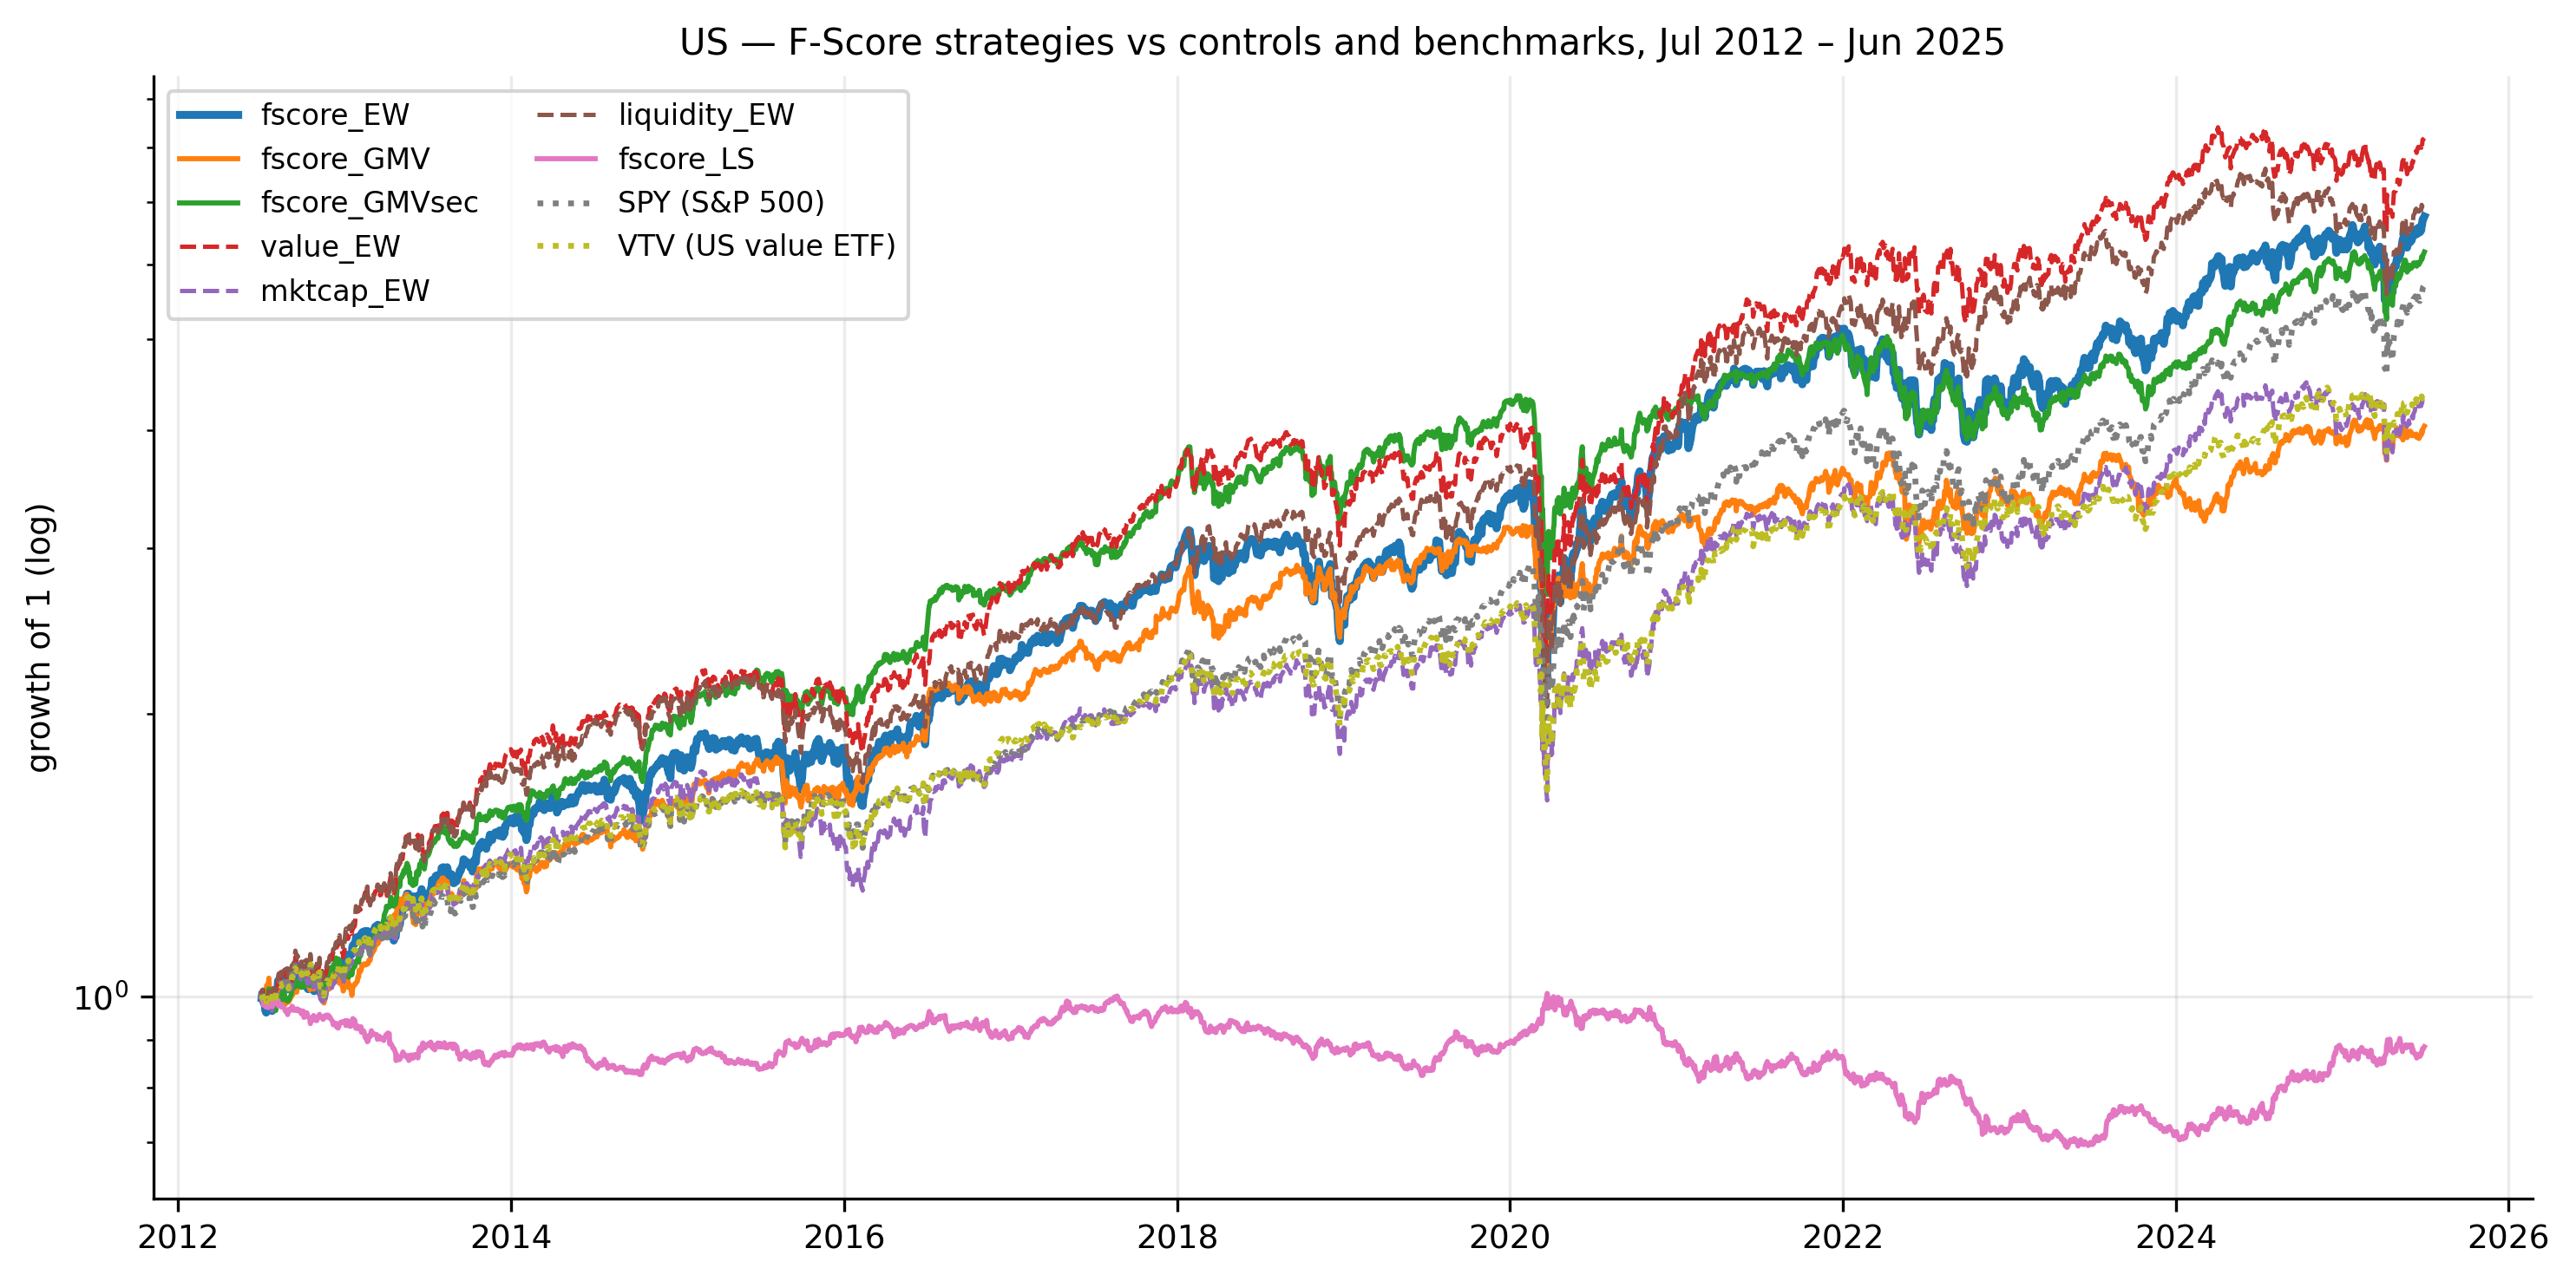
\includegraphics[width=0.9\textwidth]{fig_7_1a_us_cumulative.png}
\caption{United States cumulative performance over the common headline period.}
\label{fig:us_cumulative}
\end{figure}

\begin{figure}[H]
\centering
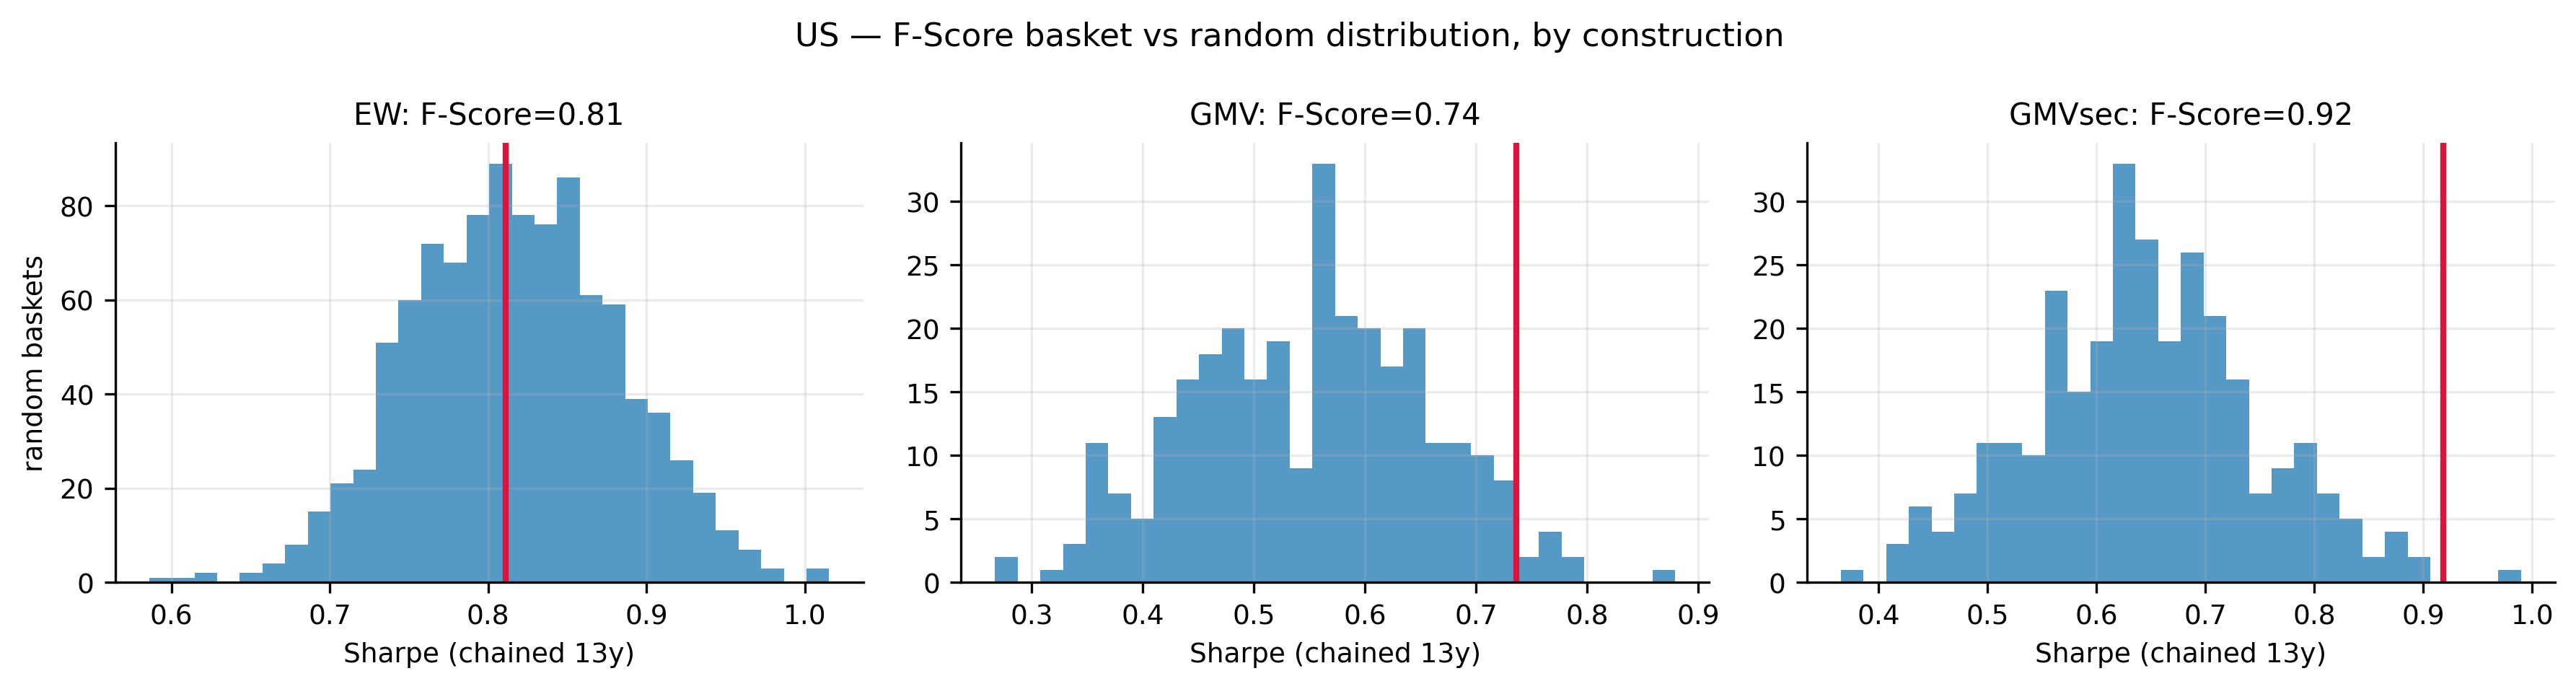
\includegraphics[width=0.96\textwidth]{fig_7_1b_us_mc_null.png}
\caption{United States F-Score portfolios placed inside their matched Monte Carlo null distributions.}
\label{fig:us_mc}
\end{figure}

\begin{figure}[H]
\centering
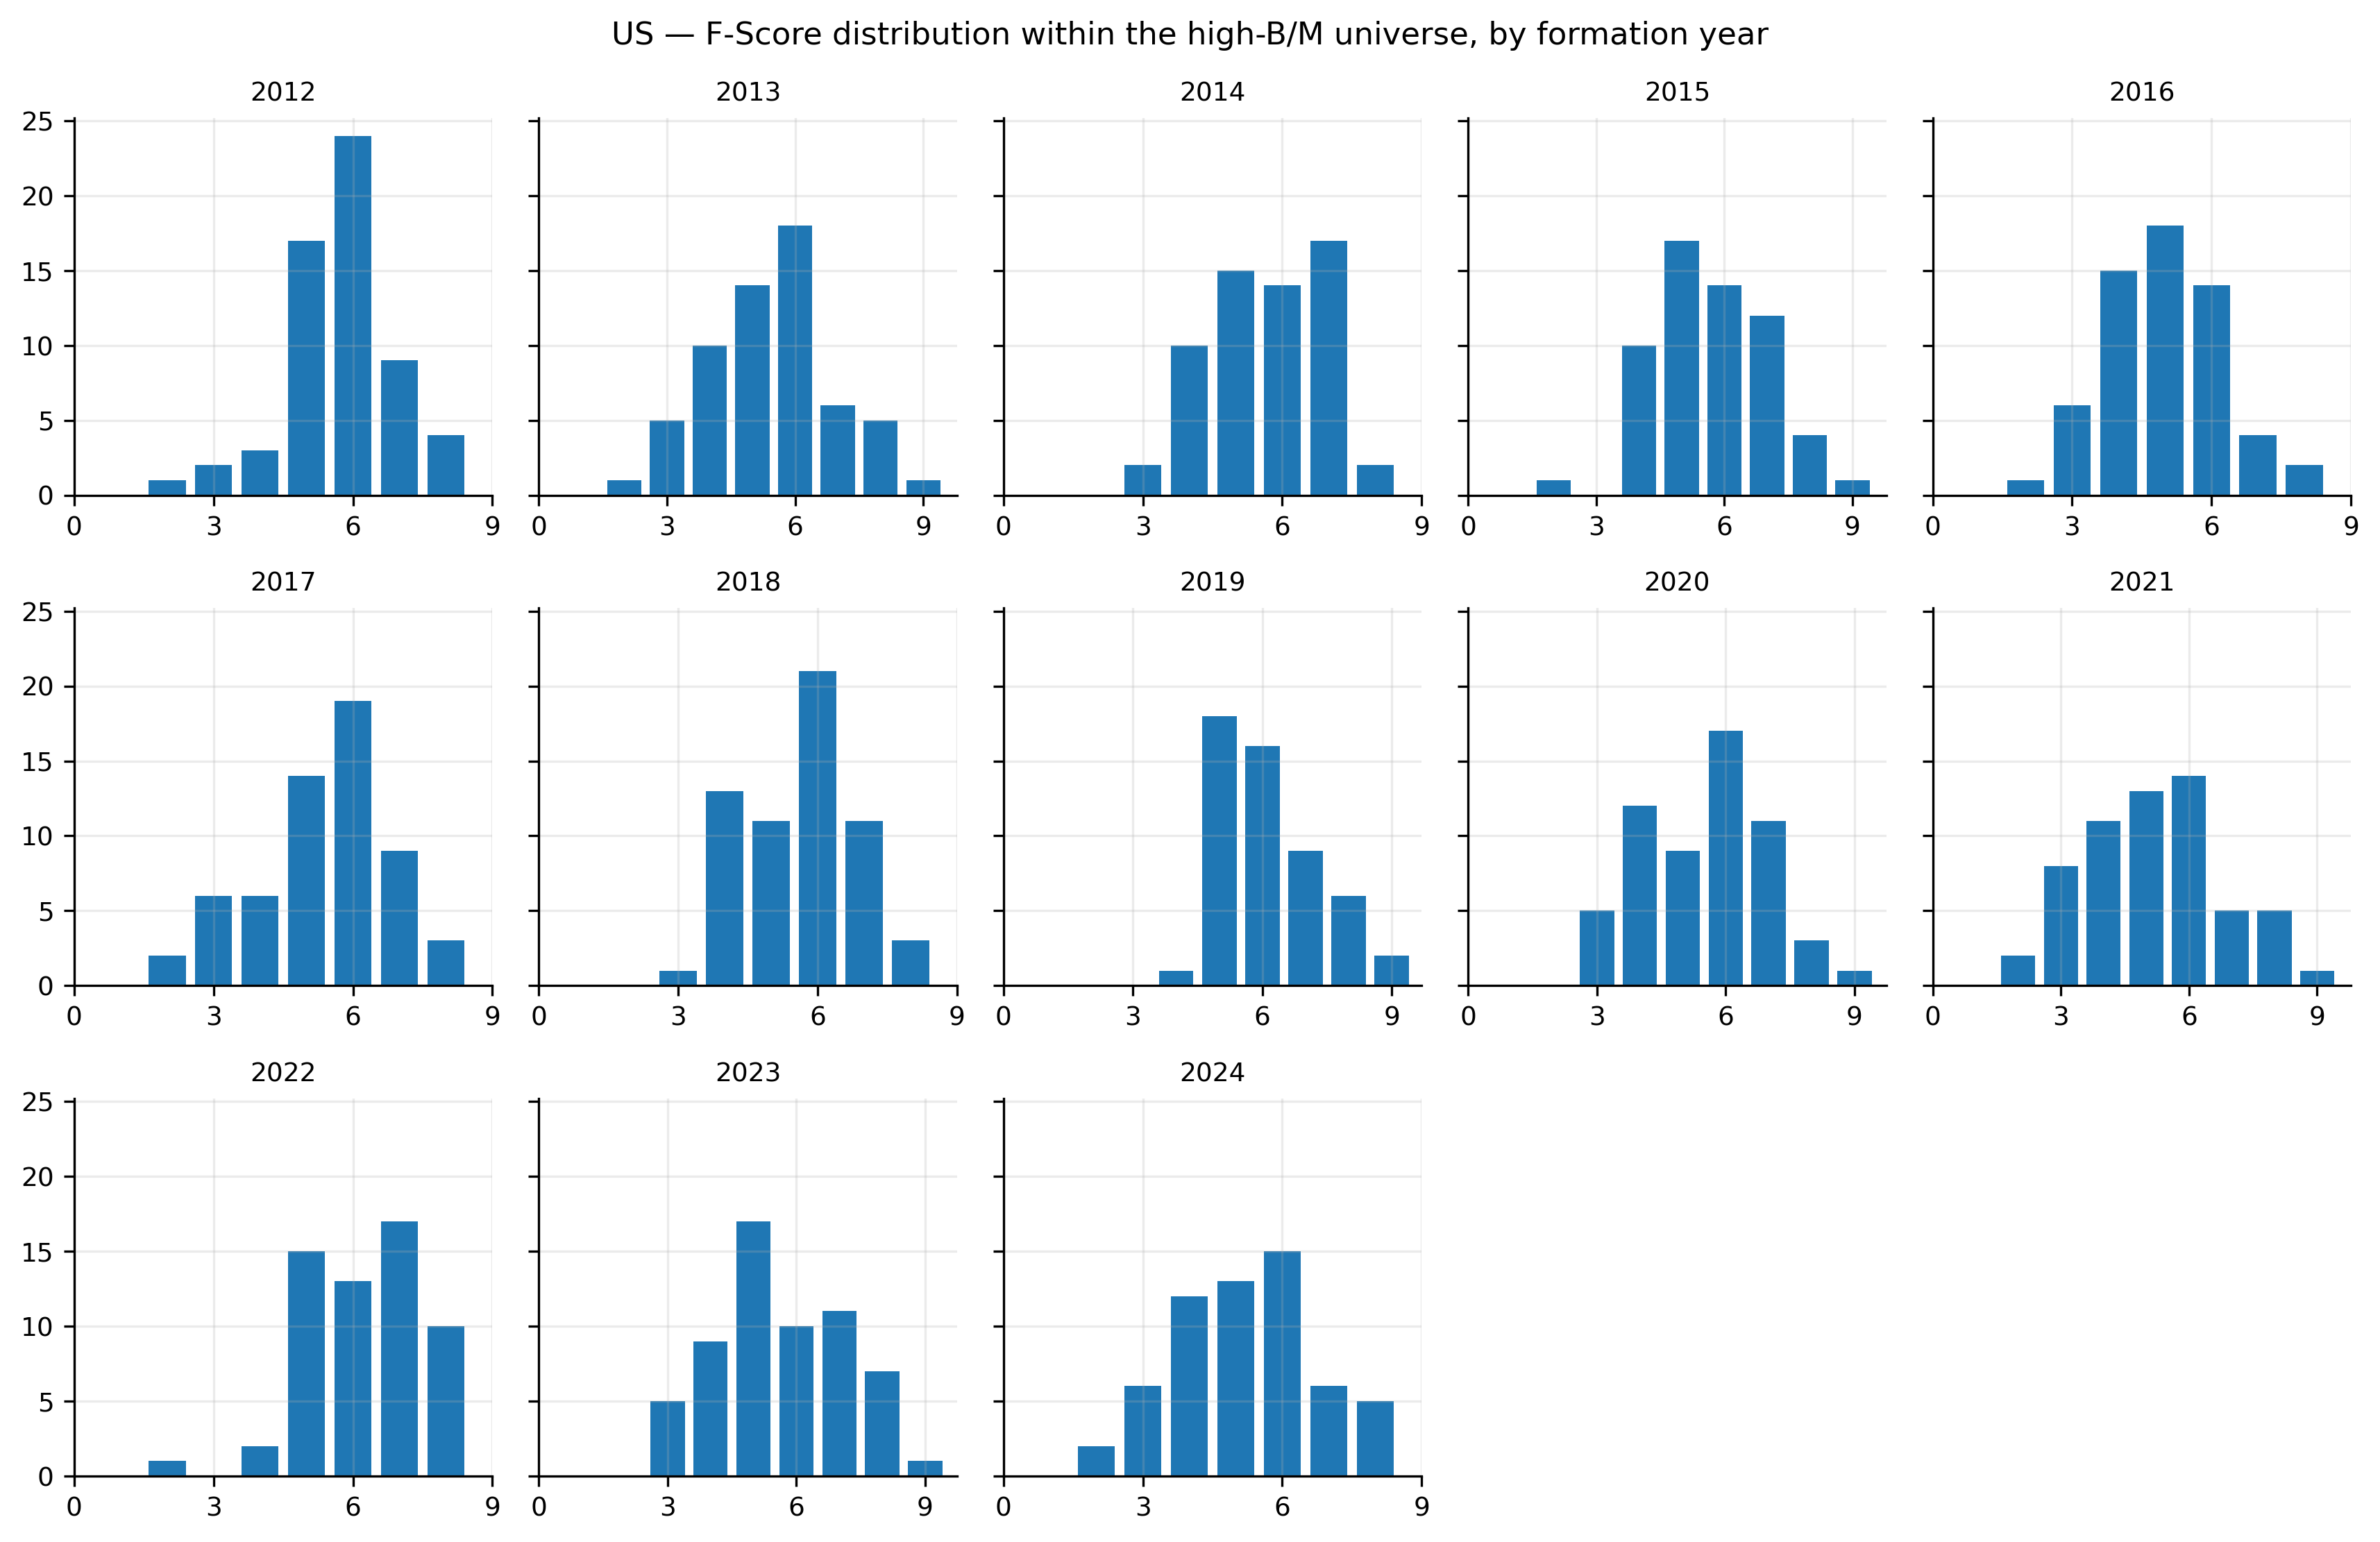
\includegraphics[width=0.9\textwidth]{fig_7_1c_us_fscore_distribution.png}
\caption{United States F-Score distribution inside the high-B/M universe by formation year.}
\label{fig:us_fscore_dist}
\end{figure}

\begin{figure}[H]
\centering
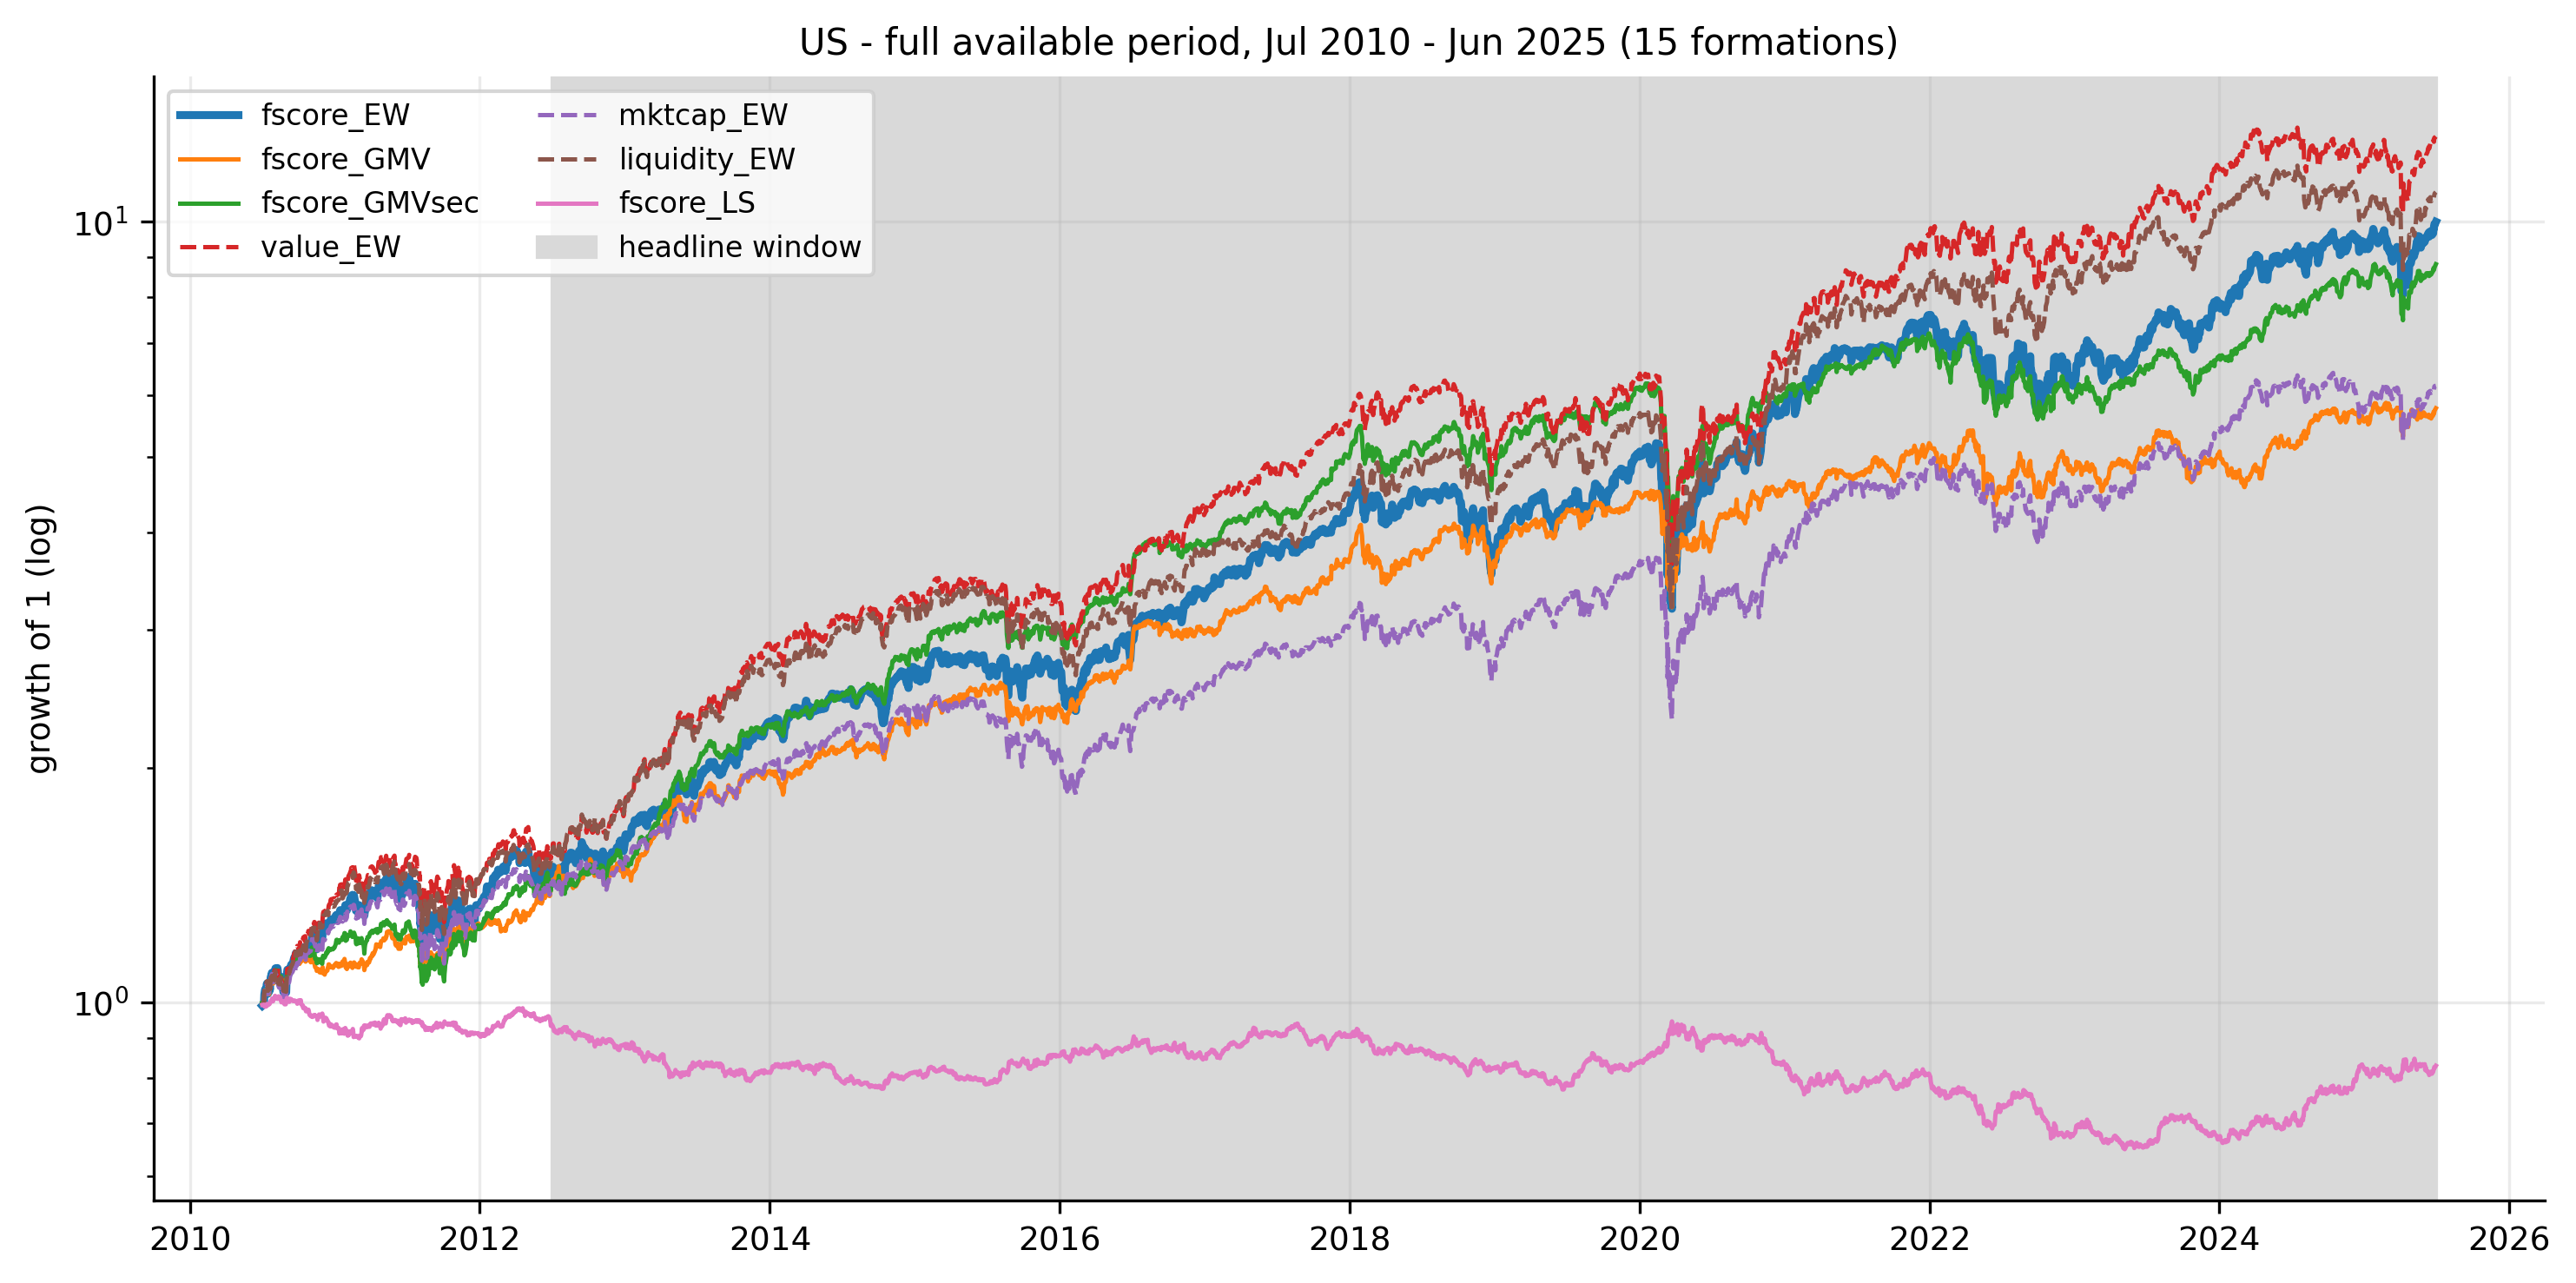
\includegraphics[width=0.9\textwidth]{fig_7_1d_us_cumulative_full.png}
\caption{United States cumulative performance over the full country-specific window.}
\label{fig:us_full}
\end{figure}

\FloatBarrier

% =============================================================================
% CHAPTER 6
% =============================================================================
\chapter{Japan Results}
\label{chap:japan}

\section{Formation Universe}

Japan is the market where the size of the opportunity set matters the most. The eligible universe is only 82 to 86 stocks in the common 2012 to 2024 period, and the high-B/M subset is therefore only 33 to 35 names. The final basket still uses $K=30$, so in many years the F-Score portfolio contains most of the high-B/M universe. This does not make the experiment invalid, but it means the ranking has much less room to separate winners from the rest than it does in the United States or Vietnam.

The F-Score distribution itself is reasonably strong in some years. The mean annual score ranges from 5.03 to 7.22, and the minimum score entering the selected basket ranges from 3 to 6. The low cutoff in some years is a direct consequence of selecting 30 names from a value set that may contain only 33 or 34 scoreable firms.

\section{Headline Performance}

The Japan equal-weight F-Score portfolio earns 15.56\% annualized with a Sharpe ratio of 0.758. Both statistics beat their matched equal-weight random distributions at the 5\% level, with $p=0.025$ for return and $p=0.032$ for Sharpe. The TOPIX ETF proxy returns 13.29\% with a Sharpe ratio of 0.682, while the Japan value ETF in USD returns 11.38\% with a Sharpe of 0.629.

The random equal-weight portfolios average 14.76\% with a very narrow standard deviation of 0.41 percentage points, and their Sharpe ratios average 0.721 with a standard deviation of 0.020. This narrow distribution makes sense because a random 30-name basket drawn from only around 33 to 35 available names overlaps heavily with every other random basket. The F-Score result is statistically significant, but the economic difference from random is still fairly modest, so both facts should be kept in mind at the same time.

\section{Effect of RMT-GMV Construction}

The RMT-GMV portfolio has a slightly lower annualized return of 15.18\% than equal weight but a higher Sharpe ratio of 0.851 because annualized volatility falls to 17.83\%. The raw risk-adjusted number therefore improves, but the matched GMV p-value for Sharpe is 0.190 and is not statistically significant. The sector-capped GMV produces a Sharpe ratio of 0.845 and a return of 15.25\%, with p-values of 0.060 and 0.067 respectively, which are close to but still above the pre-specified 5\% level.

The effective $N$ of ordinary GMV is only 5.0 and the sector-capped portfolio is 7.1. This is another example where a 30-name selection does not mean the optimized portfolio is behaving like a diversified 30-name equal-weight book. In Japan, the optimizer improves the raw Sharpe number, but the Monte Carlo evidence does not show that this improvement is unusual relative to optimized random baskets from the same small value universe.

\section{Full Japan Window}

Japan has the longest country-specific history, beginning with the July 2007 formation. Over this longer period the absolute performance numbers are lower, but the equal-weight F-Score portfolio still beats the random equal-weight distribution on annualized return and Sharpe at the 5\% level. The full-window annualized return is 6.73\% and the Sharpe ratio is 0.295. The GMV variants remain directionally better than their random averages in some metrics but do not clear the 5\% significance threshold.

\section{Interpretation}

Japan provides evidence that the F-Score ranking contains incremental information, but the result needs to be read together with the small value universe. Because $K=30$ selects almost all high-B/M names, F-Score is making a fairly small distinction between included and excluded companies. The significance is real under the matched Monte Carlo design, but it is not the same thing as saying the F-Score is creating a radically different portfolio.

This point is useful for portfolio design. A ranking signal needs enough cross-sectional room to express itself. If the eligible value universe contains only a few more names than the final basket, changing $K$ can matter more than it would in a much larger universe, and this is one reason the smaller-$K$ sensitivity run is informative even though it is not our headline specification.

\section{Japan Tables and Figures}
\label{sec:japan_exhibits}

\begin{table}[H]
\centering
\scriptsize
\caption{Formation funnel summary for Japan, common headline period.}
\label{tab:japan_funnel}
\begin{tabularx}{0.72\textwidth}{p{0.45\textwidth} X}
\hline
\textbf{Item} & \textbf{Observed range} \\
\hline
Formation years & 2012--2024 \\
Eligible universe & 82--86 \\
High-B/M set & 33--35 \\
Scoreable firms & 32--35 \\
Selected basket & 30 \\
Mean annual F-Score & 5.03--7.22 \\
Minimum F-Score entering basket & 3--6 \\
Tie-break slots per year & 1--12 \\
Delisted names in holding year & 0 \\
\hline
\end{tabularx}
\end{table}

\begin{table}[H]
\centering
\scriptsize
\caption{Japan headline performance, July 2012 to June 2025.}
\label{tab:japan_headline}

\setlength{\tabcolsep}{2.5pt}

\begin{tabular}{
@{}
M{0.21\textwidth}
M{0.13\textwidth}
M{0.09\textwidth}
M{0.12\textwidth}
M{0.13\textwidth}
M{0.09\textwidth}
M{0.06\textwidth}
@{}
}
\hline
\textbf{Portfolio} &
\textbf{Ann. return} &
\textbf{Ann. vol.} &
\textbf{Sharpe} &
\textbf{Max DD} &
\textbf{Turnover} &
\textbf{Eff. $N$} \\
\hline

F-Score, equal-weight
& \textbf{15.56\%*}
& 20.51\%
& \textbf{0.758*}
& -37.40\%
& 31.34\%
& 30.0 \\
\arrayrulecolor{gray!30}\hline\arrayrulecolor{black}

Matched random, equal-weight
& 14.76\% $\pm$ 0.41\%
& --
& 0.721 $\pm$ 0.020
& -38.71\% $\pm$ 1.14\%
& --
& -- \\
\arrayrulecolor{gray!30}\hline\arrayrulecolor{black}

F-Score, GMV (RMT-denoised)
& 15.18\%
& 17.83\%
& 0.851
& -37.77\%
& 44.83\%
& 5.0 \\
\arrayrulecolor{gray!30}\hline\arrayrulecolor{black}

Matched random, GMV
& 14.33\% $\pm$ 0.99\%
& --
& 0.799 $\pm$ 0.058
& -38.46\% $\pm$ 2.96\%
& --
& -- \\
\arrayrulecolor{gray!30}\hline\arrayrulecolor{black}

F-Score, sector-capped GMV
& 15.25\%
& 18.05\%
& 0.845
& -38.70\%
& 46.37\%
& 7.1 \\
\arrayrulecolor{gray!30}\hline\arrayrulecolor{black}

Matched random, sector-capped GMV
& 14.04\% $\pm$ 0.78\%
& --
& 0.777 $\pm$ 0.044
& -40.06\% $\pm$ 2.33\%
& --
& -- \\
\arrayrulecolor{gray!30}\hline\arrayrulecolor{black}

1306.T (TOPIX ETF, JPY)
& 13.29\%
& 19.48\%
& 0.682
& -22.82\%
& --
& -- \\
\arrayrulecolor{gray!30}\hline\arrayrulecolor{black}

EWJV (MSCI Japan Value ETF, USD)
& 11.38\%
& 18.10\%
& 0.629
& -23.32\%
& --
& -- \\

\hline
\end{tabular}

\vspace{0.05cm}

\begin{minipage}{0.98\textwidth}
\scriptsize
\textit{Note.} An asterisk marks a statistic whose matched one-sided Monte Carlo p-value is below 5\%. Benchmark rows have no turnover or effective-$N$ statistic.
\end{minipage}
\end{table}

\begin{table}[H]
\centering
\scriptsize
\caption{Japan one-sided Monte Carlo p-values for the headline F-Score constructions.}
\label{tab:japan_pvalues}
\begin{tabularx}{0.82\textwidth}{p{0.42\textwidth} X X X}
\hline
\textbf{F-Score construction} & \textbf{$p$(return)} & \textbf{$p$(Sharpe)} & \textbf{$p$(MDD)} \\
\hline
F-Score, equal-weight & 0.025 & 0.032 & 0.122 \\
F-Score, GMV (RMT-denoised) & 0.207 & 0.190 & 0.423 \\
F-Score, sector-capped GMV & 0.067 & 0.060 & 0.263 \\
\hline
\end{tabularx}
\end{table}

\begin{figure}[H]
\centering
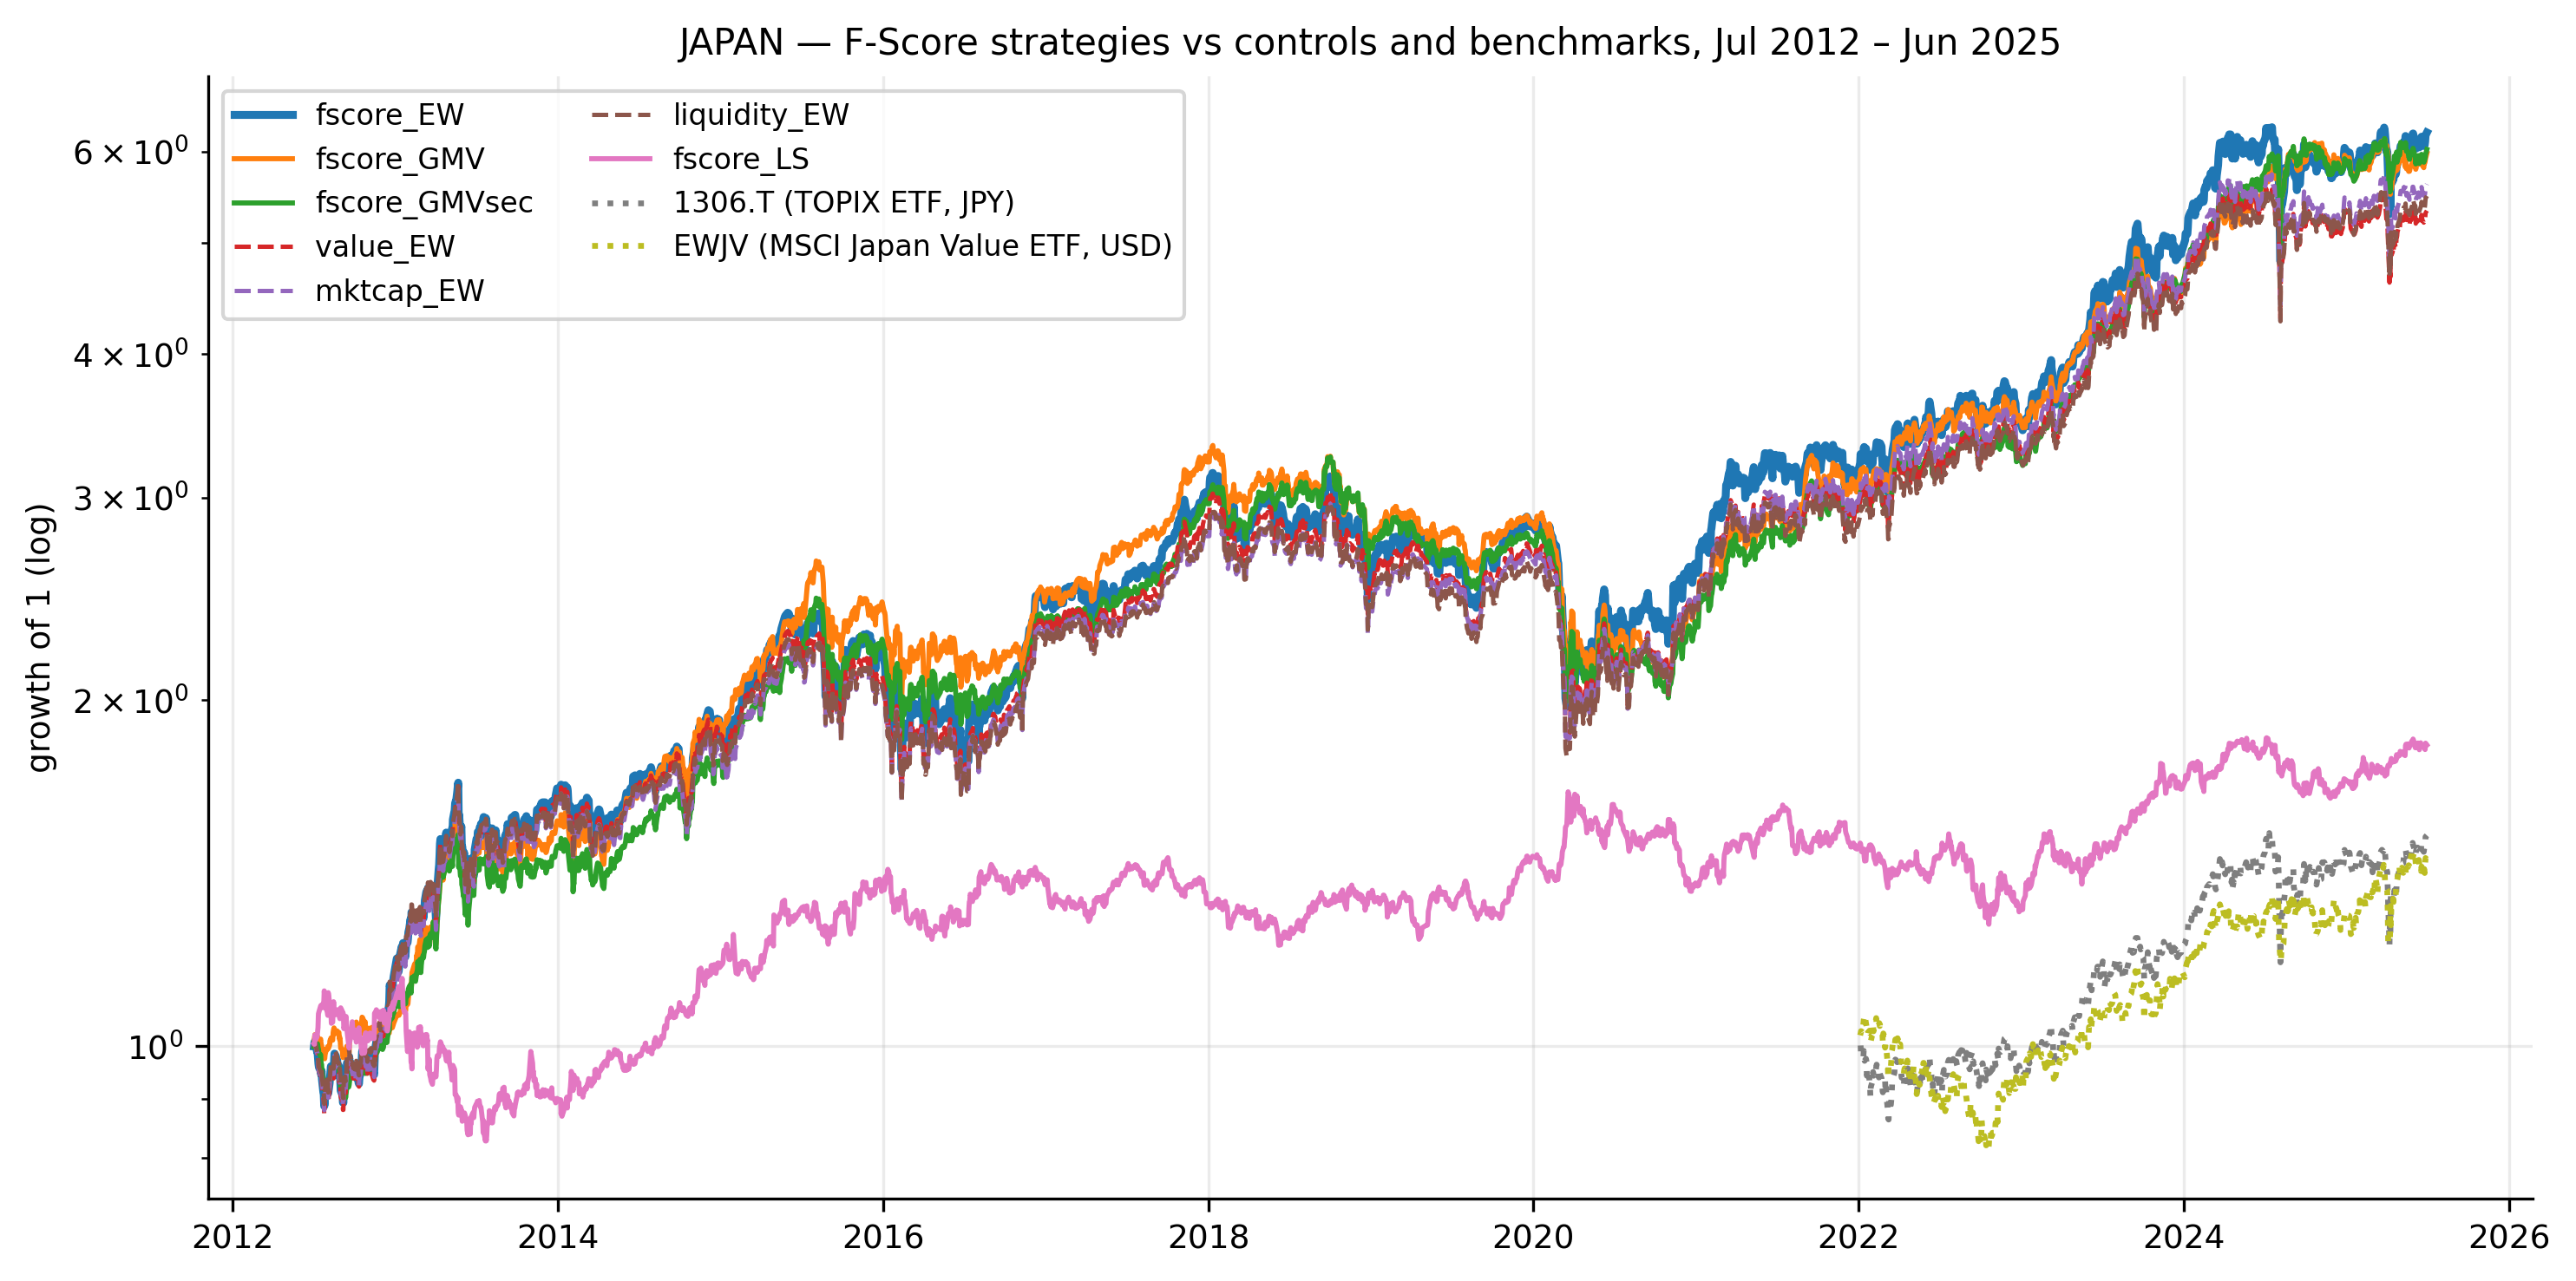
\includegraphics[width=0.9\textwidth]{fig_7_2a_japan_cumulative.png}
\caption{Japan cumulative performance over the common headline period.}
\label{fig:japan_cumulative}
\end{figure}

\begin{figure}[H]
\centering
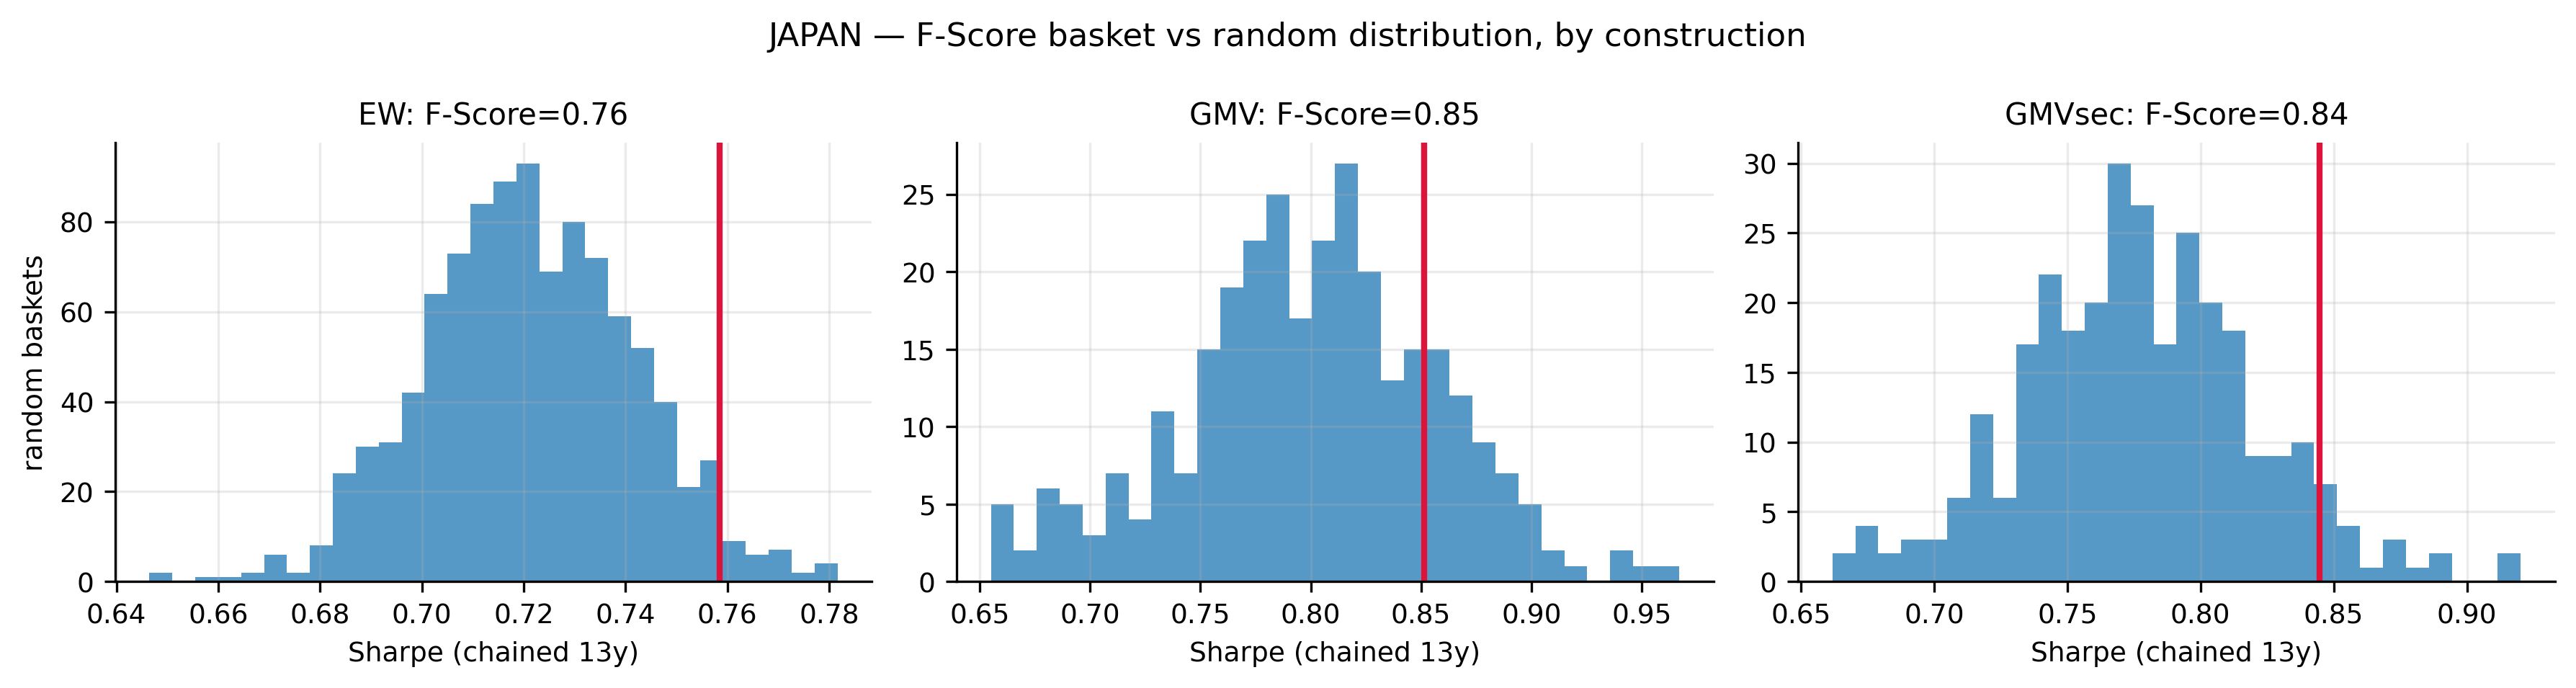
\includegraphics[width=0.9\textwidth]{fig_7_2b_japan_mc_null.png}
\caption{Japan F-Score portfolios placed inside their matched Monte Carlo null distributions.}
\label{fig:japan_mc}
\end{figure}

\begin{figure}[H]
\centering

\includegraphics[width=0.9\textwidth]{fig_7_2c_japan_fscore_distribution.png}
\caption{Japan F-Score distribution inside the high-B/M universe by formation year.}
\label{fig:japan_fscore_dist}
\end{figure}

\begin{figure}[H]
\centering
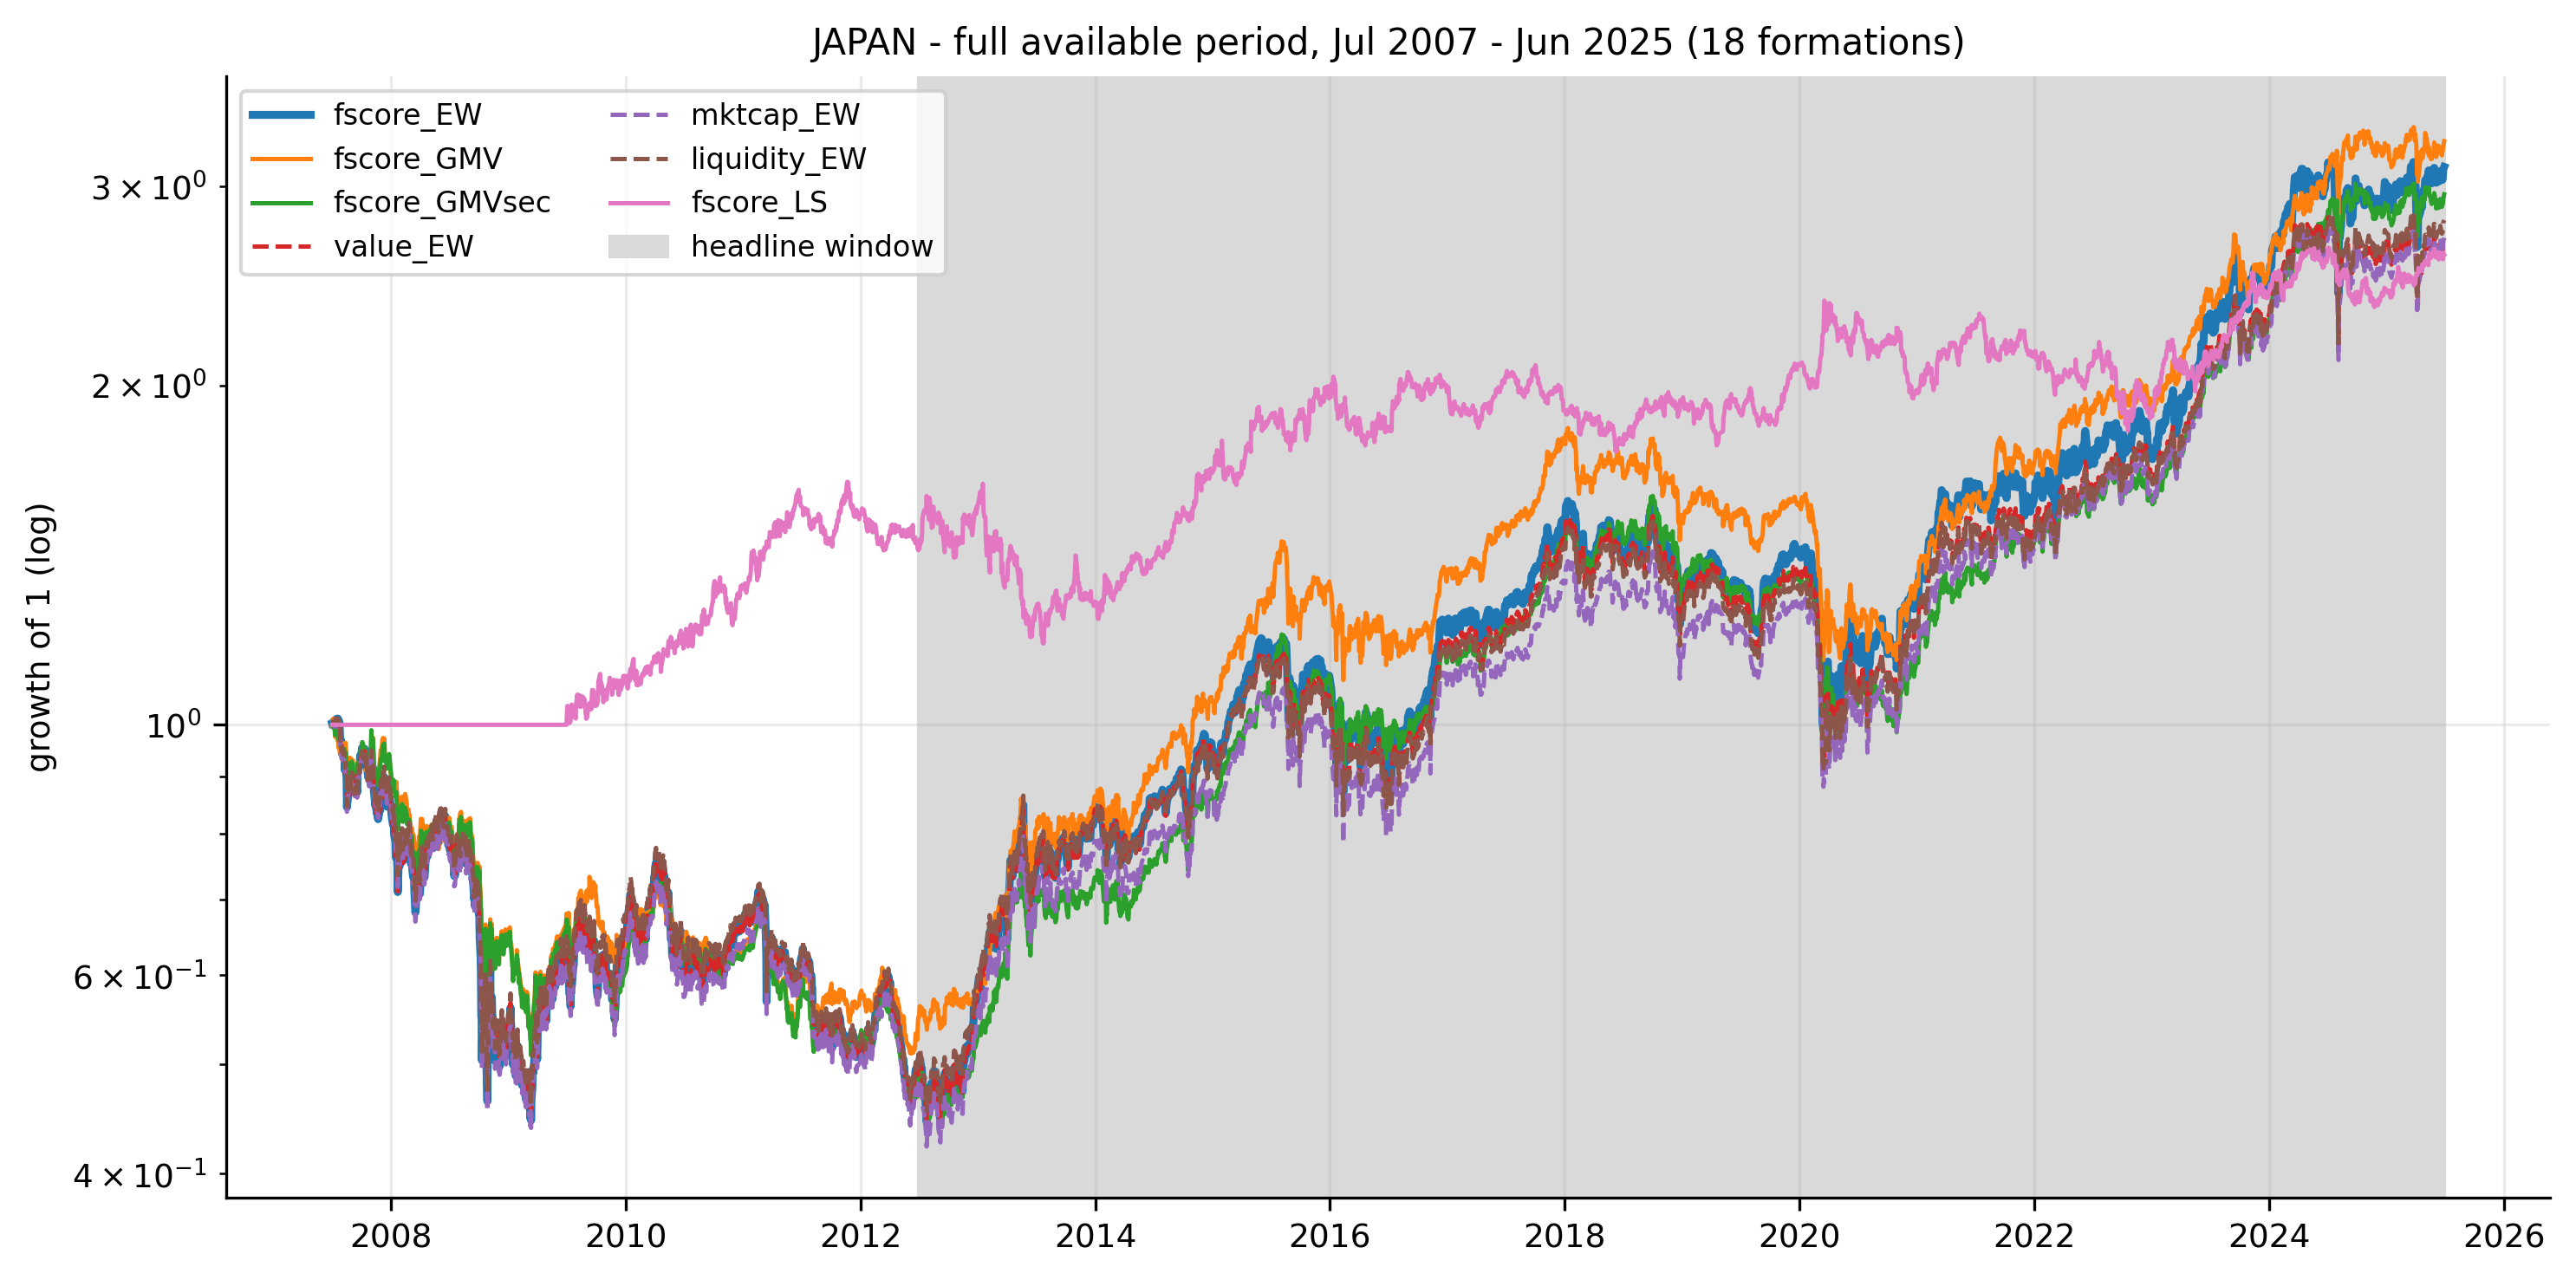
\includegraphics[width=0.96\textwidth]{fig_7_2d_japan_cumulative_full.png}
\caption{Japan cumulative performance over the full country-specific window.}
\label{fig:japan_full}
\end{figure}

\FloatBarrier

% =============================================================================
% CHAPTER 7
% =============================================================================
\chapter{Vietnam Results}
\label{chap:vietnam}

\section{Formation Universe}

Vietnam reaches the 150-name eligible-universe cap in every headline formation year, so the top 40\% high-B/M screen gives 60 names each year and all 60 have a usable score in the final funnel. The selected portfolio contains the top 30 F-Score names. The mean score ranges from 4.00 to 5.58, which is lower than the average range seen in Japan and also shows that a relative top-30 ranking does not require every selected company to have what would usually be described as a very high absolute F-Score.

Vietnam also has more holding-period delistings or names that stop printing than the other two headline funnels. The annual count ranges from zero to two. Under the common backtest convention these names are carried at their last tradable price after they stop printing, so they do not disappear and cause the portfolio to reweight itself toward survivors.

\section{Headline Performance}

The equal-weight F-Score portfolio earns 13.76\% annualized with a Sharpe ratio of 0.537. Its matched random equal-weight portfolios average 10.26\% return and a Sharpe ratio of 0.397. The one-sided p-values are 0.042 for return and 0.037 for Sharpe, so both statistics are significant at the 5\% level.

This gives Vietnam a fairly clean positive result for the selection question. The F-Score equal-weight portfolio beats VN30's 8.92\% annualized return and VNINDEX's 9.68\%, although the Sharpe ratio of 0.537 is exactly the same as the reported VNINDEX Sharpe. The benchmark comparison should be read with some care because VN30 and VNINDEX are capital indices in the available data while the portfolio returns use dividend-adjusted prices.

\section{Risk and Drawdown}

The Vietnam result also shows why return alone is not enough. The equal-weight F-Score portfolio has annualized volatility of 25.63\% and a maximum drawdown of -71.05\%. Its drawdown is somewhat better than the matched random average of -73.57\%, but the p-value is 0.091 and does not clear the headline significance threshold. The strategy therefore has a statistically interesting return and Sharpe result while still being exposed to very large peak-to-trough losses.

This is consistent with the market environment. The Vietnam portfolios are not simply lower-volatility versions of the market indices, and in fact the benchmark maximum drawdowns are much smaller than the F-Score equal-weight drawdown. An investor could therefore prefer the higher return and still find the drawdown difficult to hold in practice, which is exactly why we report both measures.

\section{Effect of RMT-GMV Construction}

The RMT-GMV portfolio raises annualized return slightly to 14.54\% and the Sharpe ratio to 0.640, while maximum drawdown improves to -59.86\%. These raw numbers look better than equal weight, but the matched optimized random distribution is much wider. The Sharpe p-value is 0.217 and the return p-value is 0.250, so we do not have statistical evidence at 5\% that the GMV construction is unusually strong compared with random high-B/M baskets passed through the same optimizer.

The sector-capped GMV is weaker in the headline Vietnam sample. Annualized return falls to 9.76\% and Sharpe to 0.416, with neither statistic significant against the matched random sector-GMV distribution. This is the opposite of the U.S. result, where the sector cap produced the strongest Monte Carlo outcome. The comparison is useful because it shows that a portfolio constraint that helps diversification in one market does not automatically improve performance in another market.

Turnover is also high in Vietnam. Equal-weight turnover is 70.66\%, while GMV and sector-capped GMV are around 90\%. The effective $N$ values of 7.4 and 9.2 again show that the optimized portfolios are much more concentrated than their nominal 30-name baskets, and their changing weights create more trading at the annual rebalance.

\section{Full Vietnam Window}

The full Vietnam window begins with the July 2011 formation. Equal-weight F-Score remains significant against its random null on return and Sharpe. The GMV portfolio becomes particularly strong in raw terms with a 19.30\% annualized return and a Sharpe ratio of 0.807, and its maximum drawdown of -54.77\% is significant against the matched random GMV distribution with $p=0.010$. Return and Sharpe remain just above the 5\% significance cutoff in this longer window, so the improvement is meaningful but we still keep the same statistical rule rather than changing the threshold after seeing it.

\section{Interpretation}

Vietnam gives the strongest general impression that F-Score selection can matter, especially because the equal-weight result is significant before any RMT covariance optimization is used. At the same time, the strategy is not low-risk and the optimized variants do not dominate uniformly. This is a good example of why our second and third research questions have to be kept separate.

The supporting $K$ sensitivity also suggests that the signal is stronger with smaller baskets in Vietnam. This could mean that the highest-ranked names contain more of the useful information and adding lower-ranked names dilutes it, but we treat that as a research clue rather than a final causal explanation. A dedicated study of portfolio size would be needed to say more.

\section{Vietnam Tables and Figures}
\label{sec:vietnam_exhibits}

\begin{table}[H]
\centering
\scriptsize
\caption{Formation funnel summary for Vietnam, common headline period.}
\label{tab:vietnam_funnel}
\begin{tabularx}{0.72\textwidth}{p{0.45\textwidth} X}
\hline
\textbf{Item} & \textbf{Observed range} \\
\hline
Formation years & 2012--2024 \\
Eligible universe & 150 \\
High-B/M set & 60 \\
Scoreable firms & 60 \\
Selected basket & 30 \\
Mean annual F-Score & 4.00--5.58 \\
Minimum F-Score entering basket & 4--6 \\
Tie-break slots per year & 4--16 \\
Delisted names in holding year & 0--2 \\
\hline
\end{tabularx}
\end{table}

\newpage

\vspace*{\fill}

\begin{table}[H]
\centering
\scriptsize
\caption{Vietnam headline performance, July 2012 to June 2025.}
\label{tab:vietnam_headline}

\setlength{\tabcolsep}{2.5pt}

\begin{tabular}{
@{}
M{0.26\textwidth}
M{0.13\textwidth}
M{0.09\textwidth}
M{0.12\textwidth}
M{0.13\textwidth}
M{0.09\textwidth}
M{0.06\textwidth}
@{}
}
\hline
\textbf{Portfolio} &
\textbf{Ann. return} &
\textbf{Ann. vol.} &
\textbf{Sharpe} &
\textbf{Max DD} &
\textbf{Turnover} &
\textbf{Eff. $N$} \\
\hline

F-Score, equal-weight
& \textbf{13.76\%*}
& 25.63\%
& \textbf{0.537*}
& -71.05\%
& 70.66\%
& 30.0 \\
\arrayrulecolor{gray!30}\hline\arrayrulecolor{black}

Matched random, equal-weight
& 10.26\% $\pm$ 2.11\%
& --
& 0.397 $\pm$ 0.082
& -73.57\% $\pm$ 1.86\%
& --
& -- \\
\arrayrulecolor{gray!30}\hline\arrayrulecolor{black}

F-Score, GMV (RMT-denoised)
& 14.54\%
& 22.72\%
& 0.640
& -59.86\%
& 90.77\%
& 7.4 \\
\arrayrulecolor{gray!30}\hline\arrayrulecolor{black}

Matched random, GMV
& 11.78\% $\pm$ 4.11\%
& --
& 0.505 $\pm$ 0.177
& -66.82\% $\pm$ 4.77\%
& --
& -- \\
\arrayrulecolor{gray!30}\hline\arrayrulecolor{black}

F-Score, sector-capped GMV
& 9.76\%
& 23.46\%
& 0.416
& -70.34\%
& 88.81\%
& 9.2 \\
\arrayrulecolor{gray!30}\hline\arrayrulecolor{black}

Matched random, sector-capped GMV
& 10.25\% $\pm$ 3.42\%
& --
& 0.430 $\pm$ 0.144
& -70.02\% $\pm$ 2.90\%
& --
& -- \\
\arrayrulecolor{gray!30}\hline\arrayrulecolor{black}

VN30 (VN30 index, VND)
& 8.92\%
& 18.81\%
& 0.474
& -48.14\%
& --
& -- \\
\arrayrulecolor{gray!30}\hline\arrayrulecolor{black}

VNINDEX (all-share index, VND)
& 9.68\%
& 18.03\%
& 0.537
& -45.26\%
& --
& -- \\

\hline
\end{tabular}

\vspace{1in}

\begin{minipage}{0.98\textwidth}
\scriptsize
\textit{Note.} An asterisk marks a statistic whose matched one-sided Monte Carlo p-value is below 5\%. Benchmark rows have no turnover or effective-$N$ statistic.
\end{minipage}
\end{table}

\begin{table}[H]
\centering
\scriptsize
\caption{Vietnam one-sided Monte Carlo p-values for the headline F-Score constructions.}
\label{tab:vietnam_pvalues}
\begin{tabularx}{0.82\textwidth}{p{0.42\textwidth} X X X}
\hline
\textbf{F-Score construction} & \textbf{$p$(return)} & \textbf{$p$(Sharpe)} & \textbf{$p$(MDD)} \\
\hline
F-Score, equal-weight & 0.042 & 0.037 & 0.091 \\
F-Score, GMV (RMT-denoised) & 0.250 & 0.217 & 0.060 \\
F-Score, sector-capped GMV & 0.540 & 0.517 & 0.570 \\
\hline
\end{tabularx}
\end{table}

\vspace*{\fill}

\newpage

\begin{figure}[H]
\centering

\includegraphics[width=0.9\textwidth]{fig_7_3a_vietnam_cumulative.png}
\caption{Vietnam cumulative performance over the common headline period.}
\label{fig:vietnam_cumulative}
\end{figure}

\begin{figure}[H]
\centering
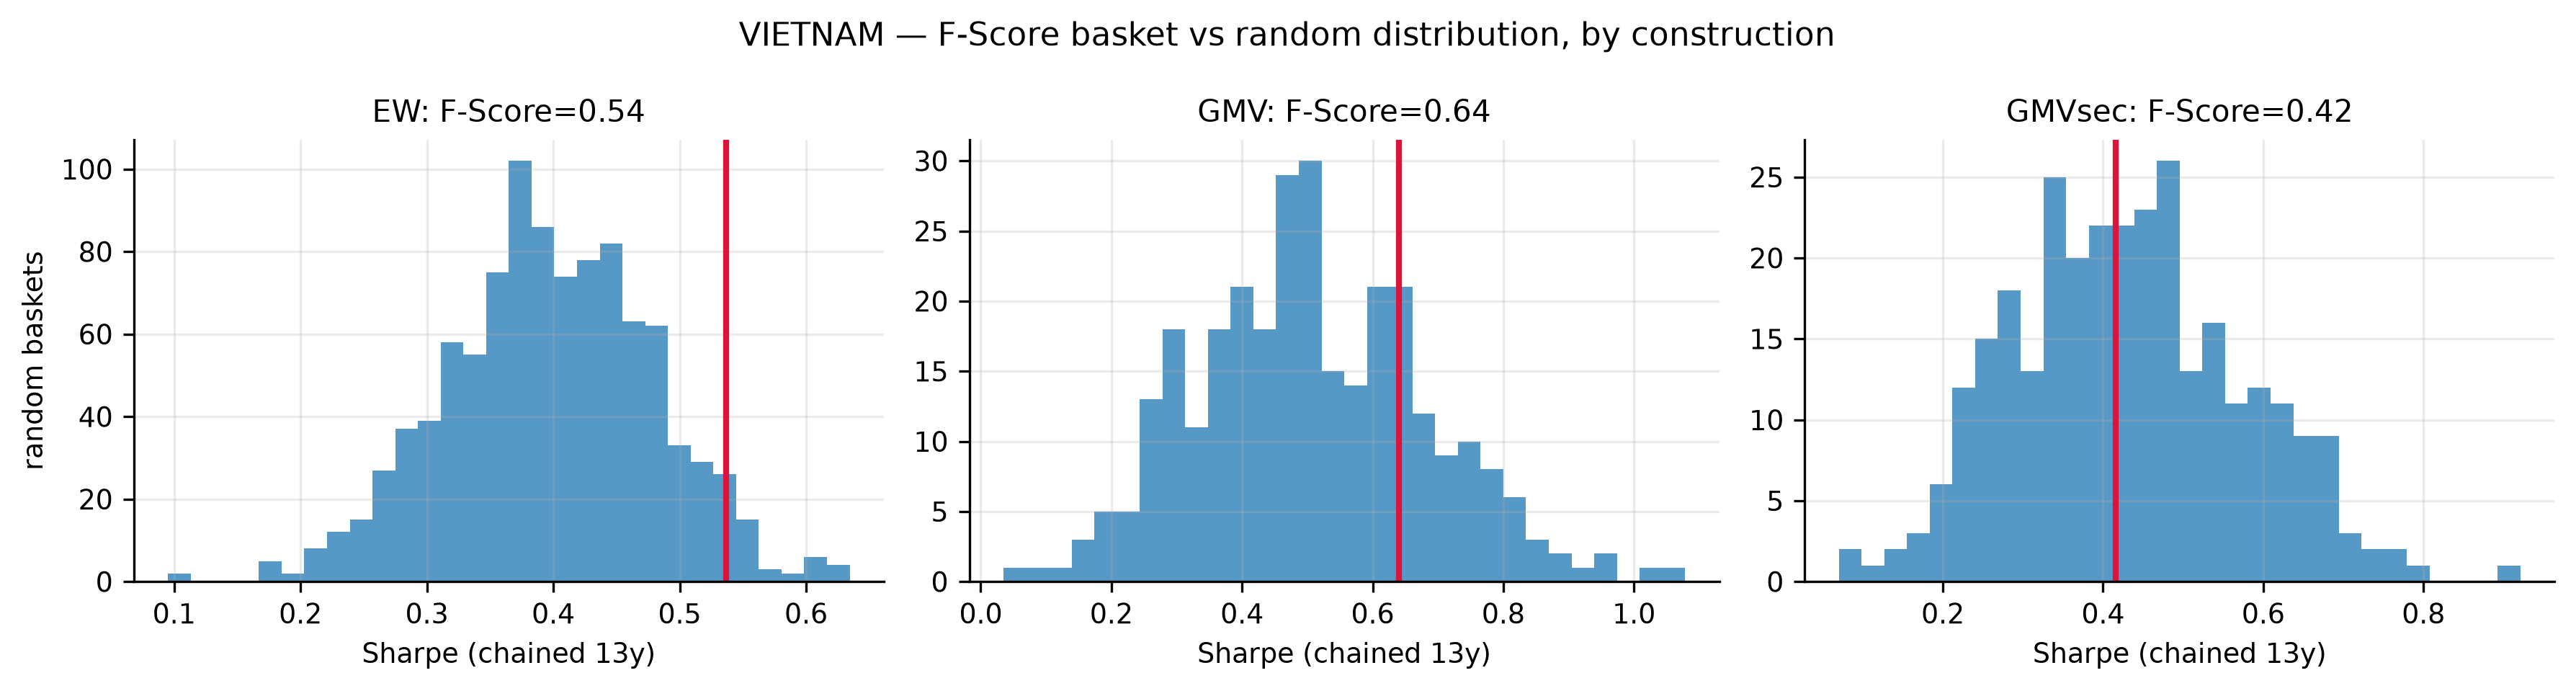
\includegraphics[width=0.9\textwidth]{fig_7_3b_vietnam_mc_null.png}
\caption{Vietnam F-Score portfolios placed inside their matched Monte Carlo null distributions.}
\label{fig:vietnam_mc}
\end{figure}

\begin{figure}[H]
\centering

\includegraphics[width=0.9\textwidth]{fig_7_3c_vietnam_fscore_distribution.png}
\caption{Vietnam F-Score distribution inside the high-B/M universe by formation year.}
\label{fig:vietnam_fscore_dist}
\end{figure}

\begin{figure}[H]
\centering

\includegraphics[width=0.96\textwidth]{fig_7_3d_vietnam_cumulative_full.png}
\caption{Vietnam cumulative performance over the full country-specific window.}
\label{fig:vietnam_full}
\end{figure}

\FloatBarrier

% =============================================================================
% CHAPTER 8
% =============================================================================
\chapter{Cross-Country Comparison}
\label{chap:crosscountry}

\section{A Common Result Does Not Appear in Every Market}

The three-country comparison does not produce one simple ranking rule that works the same way everywhere. This is not necessarily a weakness of the study because the point of adding Japan and Vietnam was partly to see whether the U.S. logic travels. Table~\ref{tab:cross_country_headline} places the three F-Score constructions side by side under the common July 2012 to June 2025 horizon.

\begin{table}[H]
\centering
\scriptsize
\caption{Cross-country comparison of the three headline F-Score constructions, July 2012 to June 2025.}
\label{tab:cross_country_headline}

\setlength{\tabcolsep}{2.5pt}

\begin{tabular}{
@{}
M{0.13\textwidth}
M{0.18\textwidth}
M{0.105\textwidth}
M{0.08\textwidth}
M{0.09\textwidth}
M{0.105\textwidth}
M{0.105\textwidth}
M{0.07\textwidth}
@{}
}
\hline
\textbf{Market} &
\textbf{Construction} &
\textbf{Ann. return} &
\textbf{Sharpe} &
\textbf{$p$(Sharpe)} &
\textbf{Max DD} &
\textbf{Turnover} &
\textbf{Eff. $N$} \\
\hline

United States
& EW
& 15.92\%
& 0.811
& 0.527
& -38.64\%
& 60.94\%
& 30.0 \\
\arrayrulecolor{gray!30}\hline\arrayrulecolor{black}

United States
& RMT-GMV
& 11.41\%
& \textbf{0.736*}
& 0.030
& \textbf{-29.11\%*}
& 60.96\%
& 5.6 \\
\arrayrulecolor{gray!30}\hline\arrayrulecolor{black}

United States
& Sector RMT-GMV
& \textbf{15.14\%*}
& \textbf{0.918*}
& 0.003
& -38.56\%
& 67.06\%
& 8.8 \\
\arrayrulecolor{gray!30}\hline\arrayrulecolor{black}

Japan
& EW
& \textbf{15.56\%*}
& \textbf{0.758*}
& 0.032
& -37.40\%
& 31.34\%
& 30.0 \\
\arrayrulecolor{gray!30}\hline\arrayrulecolor{black}

Japan
& RMT-GMV
& 15.18\%
& 0.851
& 0.190
& -37.77\%
& 44.83\%
& 5.0 \\
\arrayrulecolor{gray!30}\hline\arrayrulecolor{black}

Japan
& Sector RMT-GMV
& 15.25\%
& 0.845
& 0.060
& -38.70\%
& 46.37\%
& 7.1 \\
\arrayrulecolor{gray!30}\hline\arrayrulecolor{black}

Vietnam
& EW
& \textbf{13.76\%*}
& \textbf{0.537*}
& 0.037
& -71.05\%
& 70.66\%
& 30.0 \\
\arrayrulecolor{gray!30}\hline\arrayrulecolor{black}

Vietnam
& RMT-GMV
& 14.54\%
& 0.640
& 0.217
& -59.86\%
& 90.77\%
& 7.4 \\
\arrayrulecolor{gray!30}\hline\arrayrulecolor{black}

Vietnam
& Sector RMT-GMV
& 9.76\%
& 0.416
& 0.517
& -70.34\%
& 88.81\%
& 9.2 \\

\hline
\end{tabular}
\end{table}

The equal-weight portfolio gives the clearest answer to the F-Score selection question. It is statistically significant on return and Sharpe in Japan and Vietnam, but not in the United States. The U.S. equal-weight portfolio still has an economically respectable return, but the matched random high-B/M baskets perform similarly and the p-values are far from 5\%.

The optimized portfolios tell a different story. In the United States, RMT-GMV improves the drawdown result and the sector-capped GMV produces the strongest return and Sharpe significance. In Japan, GMV raises the raw Sharpe above equal weight but does not beat its optimized random null at 5\%. In Vietnam, GMV also improves the raw Sharpe and drawdown relative to equal weight, but the sector cap is not helpful and the optimized Monte Carlo distributions are wide enough that the headline p-values are not significant.

\section{Benchmarks Versus Statistical Nulls}

The benchmark ETFs and indices are useful for economic context, but they answer a different question from the Monte Carlo null. Table~\ref{tab:benchmark_summary} summarizes these market references. A portfolio can outperform an index and still fail to beat random value baskets, which is exactly what happens in parts of the U.S. result.

\begin{table}[H]
\centering
\scriptsize
\caption{Headline market and value benchmarks used for economic comparison.}
\label{tab:benchmark_summary}

\setlength{\tabcolsep}{3pt}

\begin{tabular}{
@{}
M{0.12\textwidth}
M{0.35\textwidth}
M{0.14\textwidth}
M{0.12\textwidth}
M{0.10\textwidth}
M{0.12\textwidth}
@{}
}
\hline
\textbf{Market} &
\textbf{Benchmark} &
\textbf{Ann. return} &
\textbf{Ann. vol.} &
\textbf{Sharpe} &
\textbf{Max DD} \\
\hline

United States
& SPY (S\&P 500)
& 14.38\%
& 16.97\%
& 0.847
& -33.72\% \\
\arrayrulecolor{gray!30}\hline\arrayrulecolor{black}

United States
& VTV (US value ETF)
& 12.10\%
& 15.99\%
& 0.756
& -36.78\% \\
\arrayrulecolor{gray!30}\hline\arrayrulecolor{black}

Japan
& 1306.T (TOPIX ETF, JPY)
& 13.29\%
& 19.48\%
& 0.682
& -22.82\% \\
\arrayrulecolor{gray!30}\hline\arrayrulecolor{black}

Japan
& EWJV (MSCI Japan Value ETF, USD)
& 11.38\%
& 18.10\%
& 0.629
& -23.32\% \\
\arrayrulecolor{gray!30}\hline\arrayrulecolor{black}

Vietnam
& VN30 (VN30 index, VND)
& 8.92\%
& 18.81\%
& 0.474
& -48.14\% \\
\arrayrulecolor{gray!30}\hline\arrayrulecolor{black}

Vietnam
& VNINDEX (all-share index, VND)
& 9.68\%
& 18.03\%
& 0.537
& -45.26\% \\

\hline
\end{tabular}
\end{table}

This distinction is one of the main lessons from the project. If we had compared only with SPY, TOPIX or VNINDEX, it would be easy to attribute every excess return to the F-Score. The matched null is stricter because it keeps the annual value universe, basket size and construction method fixed, and changes only which stocks are selected.

\section{Portfolio Concentration}

The effective number of holdings shows a consistent difference between equal weight and GMV. Equal-weight portfolios have effective $N=30$ by construction. The ordinary GMV portfolios have effective $N$ of 5.6 in the United States, 5.0 in Japan and 7.4 in Vietnam. Sector-capping raises these to 8.8, 7.1 and 9.2 respectively, but the portfolios are still much more concentrated than their nominal basket size suggests.

This concentration is not automatically bad because a minimum-variance optimizer is allowed to use small weights when they reduce estimated risk. It does mean, however, that a statement like ``we hold 30 stocks'' is incomplete for the optimized portfolios, which is why effective $N$ and turnover are reported next to the usual performance statistics.

\section{Brief Sensitivity to Basket Size and Monte Carlo Count}
\label{sec:grid_sensitivity}

The supporting grid examined $K\in\{20,25,30\}$ and larger Monte Carlo counts for the equal-weight placement test. We do not treat these as separate main experiments. The broad direction in the United States and Japan is reasonably stable, while Vietnam shows a stronger F-Score placement for $K=20$ and $K=25$ than for $K=30$. The Monte Carlo p-values in the grid are also fairly stable as $N$ increases, so the broad result is not being created by one unusually small random sample.

The three sensitivity figures are included at the end of this chapter because they are useful supporting evidence, but the conclusions in Chapters~\ref{chap:us}, \ref{chap:japan} and \ref{chap:vietnam} remain based on the frozen $K=30$ headline design with 1,000 EW and 300 optimized null simulations.

\section{Cross-Country Interpretation}

The results suggest that the value screen, the accounting signal and the portfolio optimizer are three different pieces, and their relative importance changes by market. In the United States the high-B/M environment appears strong enough that F-Score equal weighting does not distinguish itself from random value portfolios, but optimized construction can still produce a statistically unusual portfolio. Japan shows a significant equal-weight F-Score result but with a very small value universe, while Vietnam shows a stronger selection effect but also much larger drawdowns and turnover.

There is therefore no reason from our evidence to claim that one construction is always best. A more reasonable conclusion is that F-Score can contain useful fundamental information, portfolio optimization can change how that information is expressed in risk and return, and both effects depend on the market and the size of the opportunity set.

\section{Cross-Country Supporting Figures}

\begin{figure}[H]
\centering
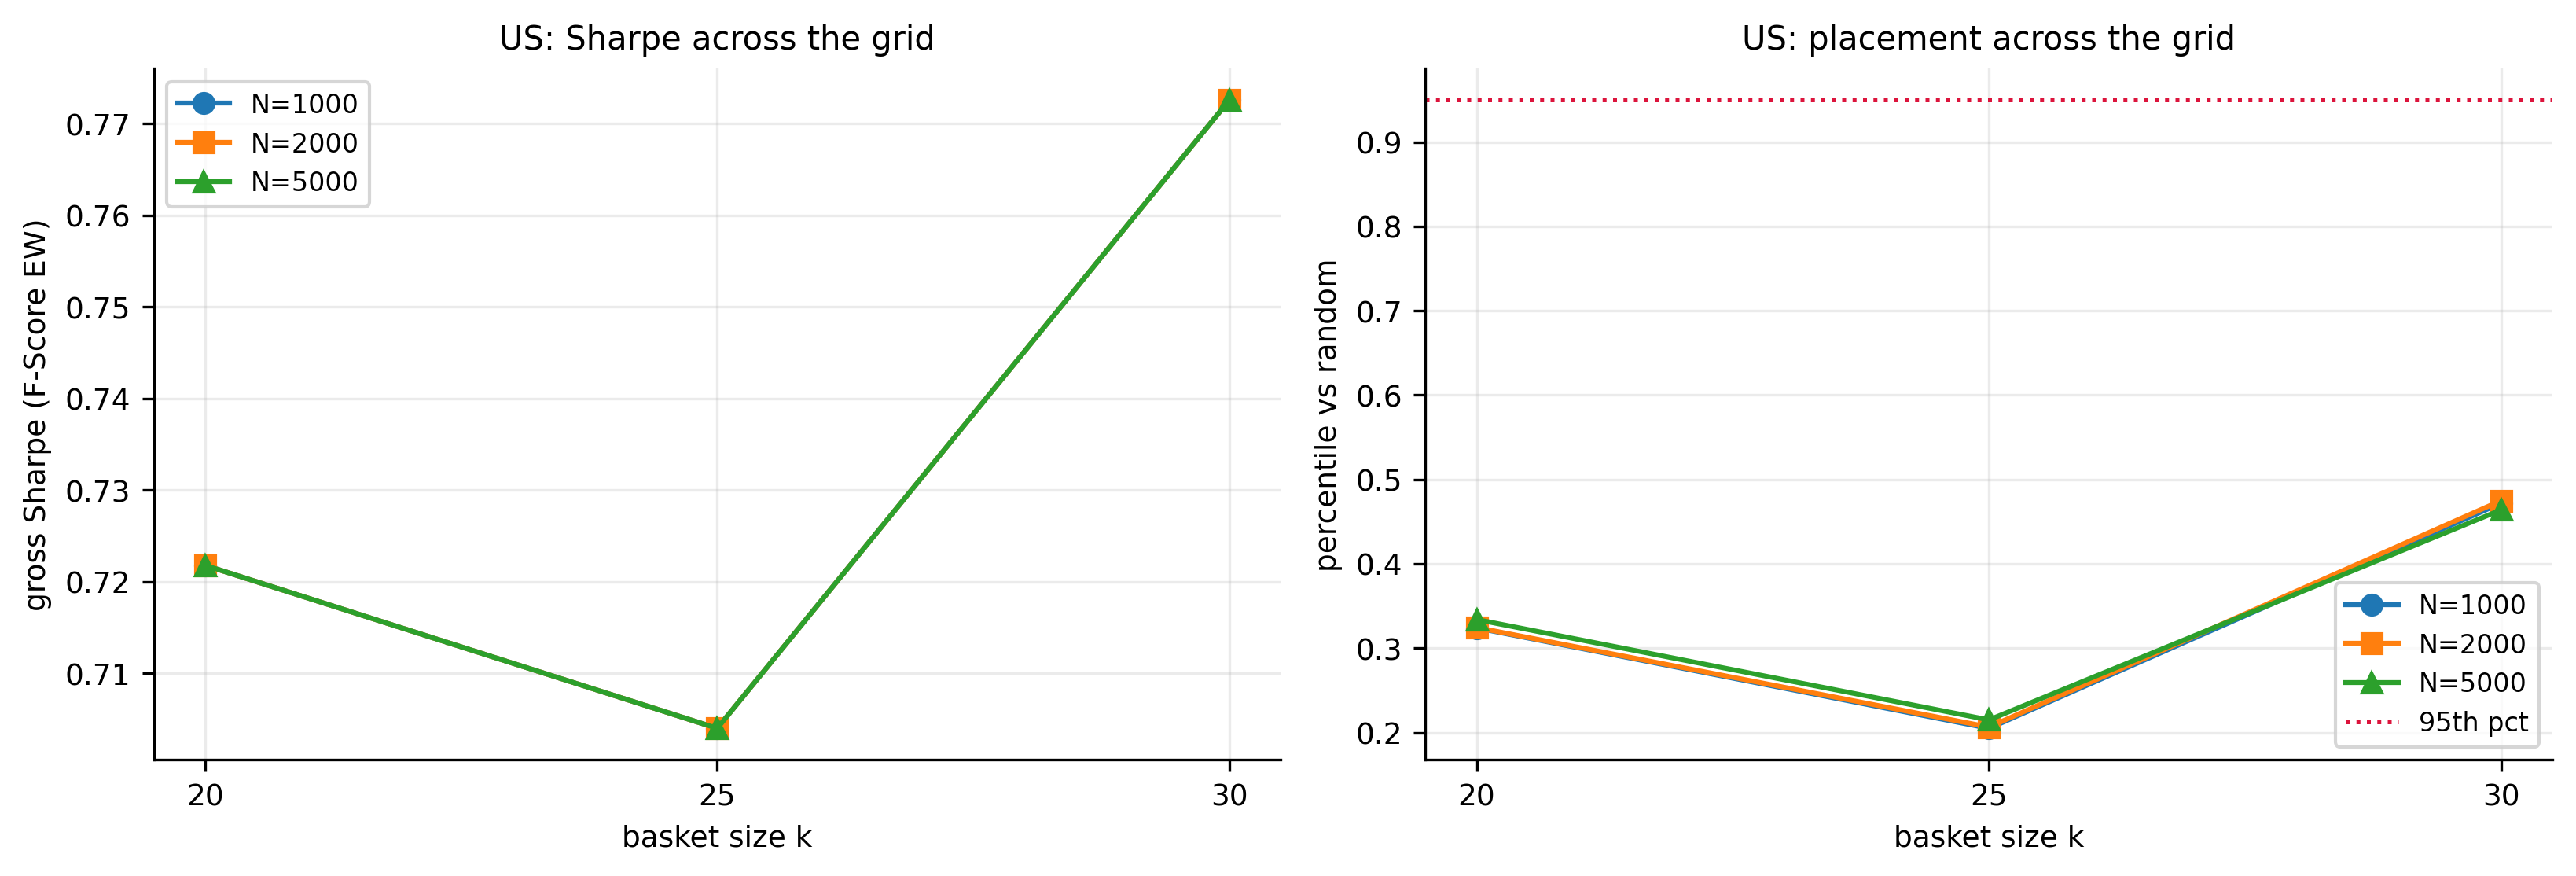
\includegraphics[width=0.96\textwidth]{fig_9_1a_us_grid_sensitivity.png}
\caption{United States sensitivity to portfolio size and Monte Carlo simulation count.}
\label{fig:us_grid}
\end{figure}

\newpage

\vspace*{\fill}

\begin{figure}[H]
\centering

\includegraphics[width=0.96\textwidth]{fig_9_1b_japan_grid_sensitivity.png}
\caption{Japan sensitivity to portfolio size and Monte Carlo simulation count.}
\label{fig:japan_grid}
\end{figure}

\vspace{0.5in}

\begin{figure}[H]
\centering
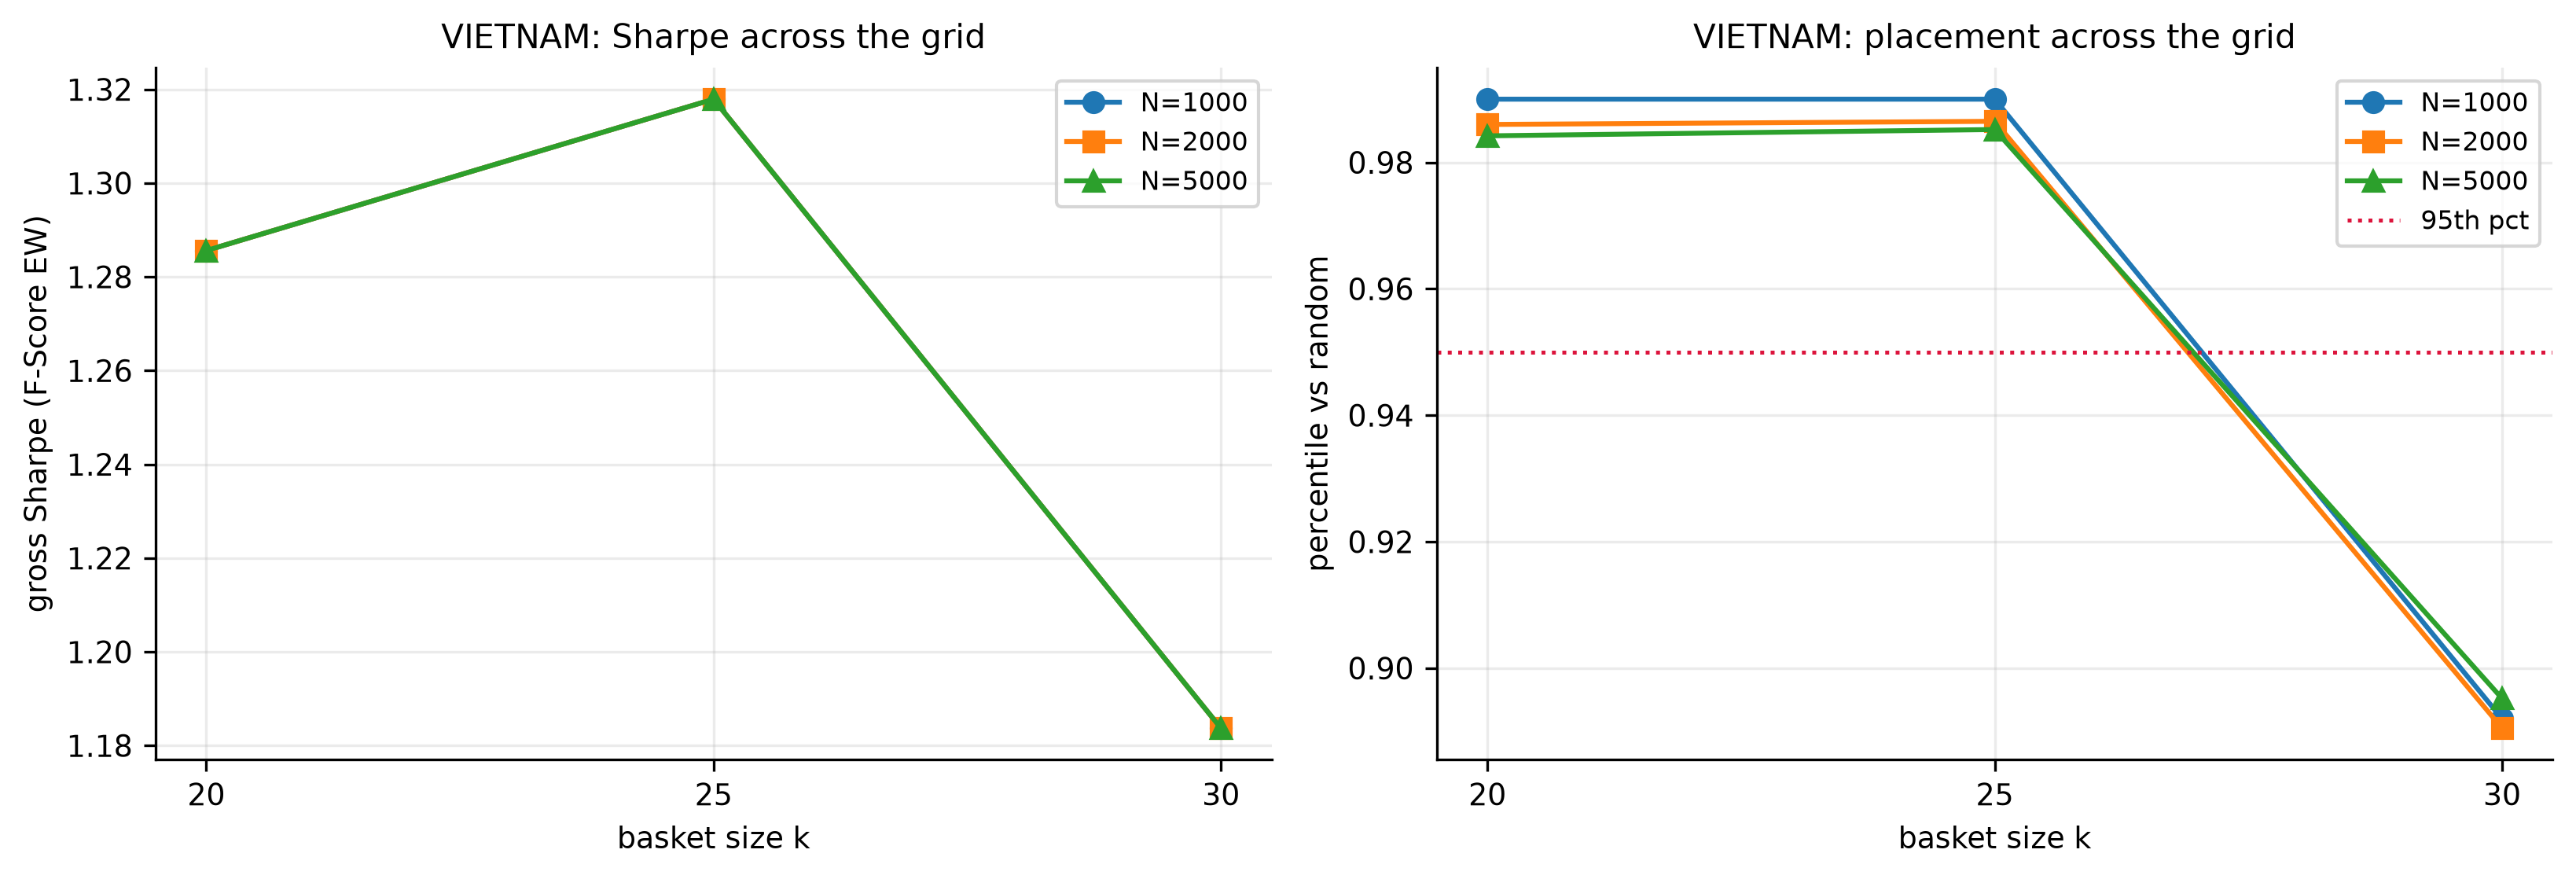
\includegraphics[width=0.96\textwidth]{fig_9_1c_vietnam_grid_sensitivity.png}
\caption{Vietnam sensitivity to portfolio size and Monte Carlo simulation count.}
\label{fig:vietnam_grid}
\end{figure}

\vspace*{\fill}

\newpage


\FloatBarrier

% =============================================================================
% CHAPTER 9
% =============================================================================
\chapter{Conclusion and Further Research}
\label{chap:conclusion}

\section{Grand Summary}

This capstone started with a simple question about whether Piotroski's F-Score can still be useful outside the setting in which it was originally studied, but the final results show that the answer depends on exactly what part of the portfolio process we are talking about. F-Score selection, high-B/M screening and minimum-variance construction are not the same source of performance, and the cross-country results make that separation fairly clear.

\begin{table}[H]
\centering
\scriptsize
\caption{Grand summary of the empirical findings.}
\label{tab:grand_summary}

\setlength{\tabcolsep}{2.5pt}

\begin{tabular}{
@{}
>{\raggedright\arraybackslash}m{0.14\textwidth}
>{\raggedright\arraybackslash}m{0.24\textwidth}
>{\raggedright\arraybackslash}m{0.24\textwidth}
>{\raggedright\arraybackslash}m{0.30\textwidth}
@{}
}
\hline

\textbf{Market} &
\textbf{F-Score selection} &
\textbf{RMT-based construction} &
\textbf{Main reading} \\
\hline

United States &
Equal-weight F-Score did not beat its matched random null at 5\%. &
GMV improved drawdown and Sharpe significance, while the sector-capped GMV had the strongest return and Sharpe evidence. &
The value universe itself was strong, and construction mattered more than F-Score ranking alone. \\
\arrayrulecolor{gray!30}\hline\arrayrulecolor{black}

Japan &
Equal-weight F-Score return and Sharpe were significant at 5\%. &
GMV raised the raw Sharpe but did not clear the 5\% Monte Carlo threshold. &
F-Score showed incremental information, but $K=30$ covers most of the small high-B/M set. \\
\arrayrulecolor{gray!30}\hline\arrayrulecolor{black}

Vietnam &
Equal-weight F-Score return and Sharpe were significant at 5\%. &
GMV improved raw risk-adjusted performance, but sector-capping was not helpful in the headline sample. &
The signal looked useful, although volatility, drawdown and turnover remained high. \\

\hline
\end{tabular}

\end{table}

For RQ1, the evidence is positive but not universal. Equal-weight F-Score selection beats the matched random high-B/M null on return and Sharpe in Japan and Vietnam, while the U.S. equal-weight result is not significant. We therefore cannot say that F-Score ranking always adds value after the high-B/M screen, but we also cannot say it has no portfolio information because two of the three markets show evidence under the same general test.

For RQ2, the effectiveness is clearly not the same across countries. The available universe, the strength of the value screen, the distribution of F-Scores, market volatility and implementation constraints are different, and the performance statistics reflect that. Japan is a particularly useful reminder that $K$ should be interpreted relative to the size of the opportunity set because 30 names is a very different choice when the high-B/M universe contains only around 34 stocks.

For RQ3, RMT-based optimization sometimes adds value but not consistently. The U.S. optimized portfolios provide the strongest statistical evidence, especially the sector-capped GMV. Japan and Vietnam obtain better raw risk-adjusted numbers from ordinary GMV in some cases, but the matched optimized nulls show that this is not automatically unusual. The equal-weight portfolios remain important because they isolate the selection question and do not use a covariance matrix or RMT at all.

\section{What We Think the Results Mean}

The main economic interpretation is that F-Score may be useful as a conditional signal rather than a universal portfolio recipe. In a market where the high-B/M screen already isolates a strong set of stocks, the incremental effect of the accounting ranking can be small. In a market where the accounting information separates firms more meaningfully, the ranking may produce a stronger shift relative to random selection. The Vietnam result is consistent with that second case, while the U.S. result looks more like the first one.

The optimizer is also not a replacement for stock selection. It changes weights using the covariance matrix and can improve volatility or drawdown even when the selected names are not statistically better than random names. This is why the U.S. result can show weak equal-weight selection evidence but stronger optimized performance, and it is also why we should not describe the whole framework as one single ``F-Score strategy.''

\section{Further Research}
\label{sec:future_work}

There are several natural extensions which follow directly from the final results.

\begin{enumerate}
    \item \textbf{Test F-Score without the high-B/M prerequisite.} The original Piotroski design gives a strong reason to begin with value stocks, but our U.S. results also suggest that the value screen itself may account for a large part of performance. A direct F-Score ranking on a broader universe would help separate these two effects.

    \item \textbf{Study detoning as an alternative covariance experiment.} The final design keeps the market mode and uses RMT denoising only. A future study could examine detoned correlation structure, but it should be designed carefully so the resulting optimization is understood as residual-risk construction rather than simply another version of the same GMV problem.

    \item \textbf{Use larger portfolio sizes and larger opportunity sets.} Portfolios with 50 or 100 names could show whether the results survive when single-stock concentration matters less. This is especially relevant in broad markets such as the United States, where a larger basket can still represent only part of the available universe.

    \item \textbf{Treat F-Score as a security-level forecasting signal.} Our study tests portfolios, not the prediction of each individual stock's future return. A useful next step would test whether F-Score predicts the cross-section of future stock returns or downside events even when the portfolio-level advantage is weak. This would address the possibility that F-Score is more useful for evaluating individual firms than for defining a fixed top-$K$ portfolio.

    \item \textbf{Extend the country set.} Malaysia remains a natural extension once consistent historical data can be assembled, and other developed, emerging and frontier markets could help show whether the Vietnam result is market-specific or part of a broader pattern.

    \item \textbf{Test alternative horizons.} The current study uses annual July formation and one-year holding periods. Different accounting lags, formation months, covariance lookbacks and holding horizons may change the balance between fundamental information and portfolio risk.

    \item \textbf{Improve market-specific implementation assumptions.} Better delisting recovery data, total-return benchmark series, deeper historical constituent files and more direct transaction-cost estimates would make the cross-country comparison closer to a live implementation.
\end{enumerate}

\section{Final Remark}

The results do not give one strategy that wins everywhere, but they do give a clearer picture of where the value may be coming from. Piotroski F-Score appears useful in some markets, high book-to-market can already be a strong filter by itself, and RMT-denoised optimization can improve the portfolio in certain settings but it is not guaranteed to do so. For us, this is a more useful conclusion than selecting only the version with the best backtest because the cross-country differences tell us what should be tested next.

% =============================================================================
% APPENDICES
% =============================================================================
\appendix

\chapter{Detailed Piotroski F-Score Definitions}
\label{app:fscore}

The main text explains the F-Score conceptually. This appendix records the nine conditions more explicitly so the reader can see how the final score is assembled. Let $t$ denote the scoring fiscal year, $t-1$ the prior fiscal year and $A_{t-1}$ beginning-of-year total assets for year $t$. Where the prior ratio needs its own beginning-of-year assets, $A_{t-2}$ is used when available.

\section{Profitability Signals}

\begin{align}
F_{\mathrm{ROA}} &= \chi\left(\frac{NI_t}{A_{t-1}}>0\right),\\
F_{\mathrm{CFO}} &= \chi\left(CFO_t>0\right),\\
F_{\Delta \mathrm{ROA}} &= \chi\left(\frac{NI_t}{A_{t-1}}>\frac{NI_{t-1}}{A_{t-2}}\right),\\
F_{\mathrm{ACCRUAL}} &= \chi\left(\frac{CFO_t}{A_{t-1}}>\frac{NI_t}{A_{t-1}}\right).
\end{align}

The last condition is an earnings-quality test. It awards a point when operating cash flow is stronger than reported net income under the same asset scaling.

\section{Leverage, Liquidity and Funding Signals}

\begin{align}
F_{\Delta \mathrm{LEV}} &= \chi\left(\frac{LTD_t}{\overline{A}_t}<\frac{LTD_{t-1}}{\overline{A}_{t-1}}\right),\\
F_{\Delta \mathrm{LIQ}} &= \chi\left(\frac{CA_t}{CL_t}>\frac{CA_{t-1}}{CL_{t-1}}\right),\\
F_{\mathrm{EQ}} &= \chi\left(\text{no new equity issuance during year }t\right).
\end{align}

In the common implementation, the equity-issuance cash-flow line is preferred where it is available, with a share-count comparison used as a fallback in data where that line is absent. The exact data mapping can therefore vary with source availability, but the economic condition is the same, which is to reward the absence of new external equity issuance.

\section{Operating Efficiency Signals}

Gross margin and asset turnover are
\begin{align}
GM_t &= \frac{Revenue_t-COGS_t}{Revenue_t},\\
ATO_t &= \frac{Revenue_t}{A_{t-1}}.
\end{align}
The two efficiency signals are
\begin{align}
F_{\Delta \mathrm{MARGIN}} &= \chi\left(GM_t>GM_{t-1}\right),\\
F_{\Delta \mathrm{TURN}} &= \chi\left(ATO_t>ATO_{t-1}\right).
\end{align}

The complete score is
\begin{equation}
\begin{aligned}
F ={}& F_{\mathrm{ROA}}+F_{\mathrm{CFO}}+F_{\Delta \mathrm{ROA}}
+F_{\mathrm{ACCRUAL}}+F_{\Delta \mathrm{LEV}} \\
&\hspace{1in}+F_{\Delta \mathrm{LIQ}}+F_{\mathrm{EQ}}
+F_{\Delta \mathrm{MARGIN}}+F_{\Delta \mathrm{TURN}}.
\end{aligned}
\end{equation}

\begin{table}[H]
\centering
\scriptsize
\caption{Detailed F-Score signal interpretation used in the study.}
\label{tab:fscore_detailed}
\begin{tabularx}{\textwidth}{p{0.20\textwidth} p{0.20\textwidth} X}
\hline
\textbf{Signal} & \textbf{Point if} & \textbf{Interpretation} \\
\hline
ROA & ROA $>0$ & Firm is profitable relative to assets. \\
CFO & CFO $>0$ & Core operations generate positive cash flow. \\
$\Delta$ROA & ROA improves & Profitability improves from the prior year. \\
Accrual quality & CFO/Assets $>$ ROA & Reported earnings are supported by operating cash flow. \\
$\Delta$Leverage & Leverage declines & Long-term balance-sheet leverage improves. \\
$\Delta$Liquidity & Current ratio rises & Short-term liquidity improves. \\
Equity issuance & No new equity issued & Firm does not rely on new equity financing in the scoring year. \\
$\Delta$Margin & Gross margin rises & Operating profitability improves. \\
$\Delta$Turnover & Asset turnover rises & Assets generate more revenue than in the prior year. \\
\hline
\end{tabularx}
\end{table}

\chapter{Full-Window Supporting Results}
\label{app:full_window}

The headline comparison uses one common period so the three countries are compared over the same formation years. This appendix records the main F-Score constructions over each country's full supported history. These are not different strategies, they are the same frozen design over the additional years available for that market.

\begin{table}[H]
\centering
\scriptsize
\caption{Full-window F-Score performance for the country-specific sample periods.}
\label{tab:full_window_appendix}

\setlength{\tabcolsep}{2.5pt}

\begin{tabular}{
@{}
M{0.13\textwidth}
M{0.18\textwidth}
M{0.105\textwidth}
M{0.09\textwidth}
M{0.10\textwidth}
M{0.11\textwidth}
M{0.10\textwidth}
@{}
}
\hline
\textbf{Market} &
\textbf{Construction} &
\textbf{Ann. return} &
\textbf{Sharpe} &
\textbf{$p$(Sharpe)} &
\textbf{Max DD} &
\textbf{$p$(MDD)} \\
\hline

United States
& EW
& 16.68\%
& 0.849
& 0.569
& -38.64\%
& 0.102 \\
\arrayrulecolor{gray!30}\hline\arrayrulecolor{black}

United States
& RMT-GMV
& 12.46\%
& \textbf{0.815*}
& 0.040
& \textbf{-29.11\%*}
& 0.040 \\
\arrayrulecolor{gray!30}\hline\arrayrulecolor{black}

United States
& Sector RMT-GMV
& \textbf{15.71\%*}
& \textbf{0.957*}
& 0.020
& -38.56\%
& 0.477 \\
\arrayrulecolor{gray!30}\hline\arrayrulecolor{black}

Japan
& EW
& \textbf{6.73\%*}
& \textbf{0.295*}
& 0.039
& -56.13\%
& 0.190 \\
\arrayrulecolor{gray!30}\hline\arrayrulecolor{black}

Japan
& RMT-GMV
& 7.05\%
& 0.366
& 0.137
& -49.48\%
& 0.130 \\
\arrayrulecolor{gray!30}\hline\arrayrulecolor{black}

Japan
& Sector RMT-GMV
& 6.39\%
& 0.328
& 0.120
& -56.36\%
& 0.777 \\
\arrayrulecolor{gray!30}\hline\arrayrulecolor{black}

Vietnam
& EW
& \textbf{11.67\%*}
& \textbf{0.446*}
& 0.042
& -70.44\%
& 0.100 \\
\arrayrulecolor{gray!30}\hline\arrayrulecolor{black}

Vietnam
& RMT-GMV
& 19.30\%
& 0.807
& 0.067
& \textbf{-54.77\%*}
& 0.010 \\
\arrayrulecolor{gray!30}\hline\arrayrulecolor{black}

Vietnam
& Sector RMT-GMV
& 13.07\%
& 0.545
& 0.380
& -67.04\%
& 0.320 \\

\hline
\end{tabular}
\end{table}

% =============================================================================
% REFERENCES
% =============================================================================
\chapter*{References}
\addcontentsline{toc}{chapter}{References}

\begin{hangparas}{0.5in}{1}

Bloomberg L.P. (2026). \textit{Bloomberg Terminal} [Computer software and financial database]. Bloomberg L.P.

Fama, E. F., \& French, K. R. (1992). The cross-section of expected stock returns. \textit{The Journal of Finance, 47}(2), 427--465. \url{https://doi.org/10.1111/j.1540-6261.1992.tb04398.x}

Laloux, L., Cizeau, P., Bouchaud, J.-P., \& Potters, M. (1999). Noise dressing of financial correlation matrices. \textit{Physical Review Letters, 83}(7), 1467--1470. \url{https://doi.org/10.1103/PhysRevLett.83.1467}

L\'opez de Prado, M. (2018). \textit{Advances in financial machine learning}. Wiley.

Marchenko, V. A., \& Pastur, L. A. (1967). Distribution of eigenvalues for some sets of random matrices. \textit{Mathematics of the USSR-Sbornik, 1}(4), 457--483. \url{https://doi.org/10.1070/SM1967v001n04ABEH001994}

Markowitz, H. (1952). Portfolio selection. \textit{The Journal of Finance, 7}(1), 77--91. \url{https://doi.org/10.1111/j.1540-6261.1952.tb01525.x}

Piotroski, J. D. (2000). Value investing: The use of historical financial statement information to separate winners from losers. \textit{Journal of Accounting Research, 38}, 1--41. \url{https://doi.org/10.2307/2672906}

Plerou, V., Gopikrishnan, P., Rosenow, B., Amaral, L. A. N., \& Stanley, H. E. (1999). Universal and nonuniversal properties of cross correlations in financial time series. \textit{Physical Review Letters, 83}(7), 1471--1474. \url{https://doi.org/10.1103/PhysRevLett.83.1471}

Sharpe, W. F. (1966). Mutual fund performance. \textit{The Journal of Business, 39}(1), 119--138. \url{https://doi.org/10.1086/294846}

U.S. Securities and Exchange Commission. (2026). \textit{EDGAR company filings database} [Data set].

Yahoo Finance. (2026). \textit{Historical market data} [Data set].

FireAnt. (2026). \textit{Vietnam equity market and corporate data} [Data set].

CafeF. (2026). \textit{Vietnam corporate and market data} [Data set].

TCBS. (2026). \textit{Vietnam securities market data} [Data set].

\end{hangparas}

\end{document}
